
\documentclass{article} % For LaTeX2e
\usepackage{iclr2025_conference,times}

\theoremstyle{plain}
\newtheorem{theorem}{Theorem}
\newtheorem{lemma}{Lemma}[section]
\newtheorem{proposition}[lemma]{Proposition}
\newtheorem{corollary}[lemma]{Corollary}
\theoremstyle{definition}
\newtheorem{definition}[lemma]{Definition}
\newtheorem{assumption}[lemma]{Assumption}
\theoremstyle{remark}
\newtheorem{remark}[lemma]{Remark}


\newcommand{\diag}{\mathrm{diag}}
\newcommand{\norm}[1]{\left\|{#1}\right\|} %
\newcommand{\rank}{\mathrm{rank}}
\newcommand{\B}{\mathcal{B}}
\newcommand{\M}{\mathcal{M}}
\newcommand{\BS}{\B^*}
\newcommand{\BBS}{\B\B^*}
\newcommand{\BSB}{\B^*\B}
\newcommand{\MMS}{\M\M^*}
\newcommand{\MSM}{\M^*\M}
\newcommand{\BF}{\mathcal{B}\mathcal{F}}
\newcommand{\BD}{\mathcal{B}\mathcal{D}}
\newcommand{\DB}{\mathcal{D}\mathcal{B}}
\newcommand{\ind}[1]{^{(#1)}}

\newcommand{\vzero}{\mathbf{0}}
\newcommand{\vone}{\mathbf{1}}
\newcommand{\va}{\mathbf{a}}
\newcommand{\vb}{\mathbf{b}}
\newcommand{\vc}{\mathbf{c}}
\newcommand{\vd}{\mathbf{d}}
\newcommand{\ve}{\mathbf{e}}
\newcommand{\vf}{\mathbf{f}}
\newcommand{\vg}{\mathbf{g}}
\newcommand{\vh}{\mathbf{h}}
\newcommand{\vi}{\mathbf{i}}
\newcommand{\vj}{\mathbf{j}}
\newcommand{\vk}{\mathbf{k}}
\newcommand{\vl}{\mathbf{l}}
\newcommand{\vm}{\mathbf{m}}
\newcommand{\vn}{\mathbf{n}}
\newcommand{\vo}{\mathbf{o}}
\newcommand{\vp}{\mathbf{p}}
\newcommand{\vq}{\mathbf{q}}
\newcommand{\vr}{\mathbf{r}}
\newcommand{\vs}{\mathbf{s}}
\newcommand{\vt}{\mathbf{t}}
\newcommand{\vu}{\mathbf{u}}
\newcommand{\vv}{\mathbf{v}}
\newcommand{\vw}{\mathbf{w}}
\newcommand{\vx}{\mathbf{x}}
\newcommand{\vy}{\mathbf{y}}
\newcommand{\vz}{\mathbf{z}}
\newcommand{\vA}{\mathbf{A}}
\newcommand{\vB}{\mathbf{B}}
\newcommand{\vC}{\mathbf{C}}
\newcommand{\vD}{\mathbf{D}}
\newcommand{\vE}{\mathbf{E}}
\newcommand{\vF}{\mathbf{F}}
\newcommand{\vG}{\mathbf{G}}
\newcommand{\vH}{\mathbf{H}}
\newcommand{\vI}{\mathbf{I}}
\newcommand{\vJ}{\mathbf{J}}
\newcommand{\vK}{\mathbf{K}}
\newcommand{\vL}{\mathbf{L}}
\newcommand{\vM}{\mathbf{M}}
\newcommand{\vN}{\mathbf{N}}
\newcommand{\vO}{\mathbf{O}}
\newcommand{\vP}{\mathbf{P}}
\newcommand{\vQ}{\mathbf{Q}}
\newcommand{\vR}{\mathbf{R}}
\newcommand{\vS}{\mathbf{S}}
\newcommand{\vT}{\mathbf{T}}
\newcommand{\vU}{\mathbf{U}}
\newcommand{\vV}{\mathbf{V}}
\newcommand{\vW}{\mathbf{W}}
\newcommand{\vX}{\mathbf{X}}
\newcommand{\vY}{\mathbf{Y}}
\newcommand{\vZ}{\mathbf{Z}}

\newcommand{\cA}{\mathcal{A}}
\newcommand{\cB}{\mathcal{B}}
\newcommand{\cC}{\mathcal{C}}
\newcommand{\cD}{\mathcal{D}}
\newcommand{\cF}{\mathcal{F}}
\newcommand{\cG}{\mathcal{G}}
\newcommand{\cH}{\mathcal{H}}
\newcommand{\cI}{\mathcal{I}}
\newcommand{\cK}{\mathcal{K}}
\newcommand{\cL}{\mathcal{L}}
\newcommand{\cM}{\mathcal{M}}
\newcommand{\cN}{\mathcal{N}}
\newcommand{\cP}{\mathcal{P}}
\newcommand{\cS}{\mathcal{S}}
\newcommand{\cT}{\mathcal{T}}
\newcommand{\cX}{\mathcal{X}}

\newcommand{\R}{\mathbb{R}}
\newcommand{\F}{\mathbb{F}}

\newcommand{\Z}{\mathbb{Z}}
\newcommand{\ep}{\epsilon}
\newcommand{\g}{\gamma}
\newcommand{\Y}{\infty}
\newcommand{\f}[2]{\dfrac{#1}{#2}}
\newcommand{\ff}[2]{\tfrac{#1}{#2}}
\newcommand{\lm}[2]{\lim_{#1\rightarrow #2}}
\newcommand{\de}{\delta}
\newcommand{\T}{\theta}
\newcommand{\tm}{\times}
\newcommand{\su}[2]{\mathlarger{\sum\limits_{#1}^{#2}}}
\newcommand{\pd}[2]{\mathlarger{\prod\limits_{#1}^{#2}}}
\renewcommand{\sec}[1]{\section*{#1}}
\newcommand{\st}[1]{\subsection*{#1}}
\newcommand{\sst}[1]{\subsubsection*{#1}}
\renewcommand{\b}{\textbf}
\newcommand{\lessim}{\lesssim}
\newcommand{\E}{\mathbb{E}}
\newcommand{\p}{\partial}
\newcommand{\lt}{\left(}
\newcommand{\rt}{\right)}
\newcommand{\Lt}{\left[}
\newcommand{\Rt}{\right]}
\newcommand{\A}{\alpha}
\renewcommand{\b}{\beta}
\newcommand{\I}[2]{\mathlarger{\int_{#1}^{#2}}}
\newcommand{\G}{\nabla}
\newcommand{\Om}{\Omega}
\newcommand{\y}{\tau}
\newcommand{\K}{\mathcal{K}}
\newcommand{\C}{\mathbb{C}}
\newcommand{\om}{\omega}
\newcommand{\D}{\Delta}
\newcommand{\N}{\mathcal{N}}
\newcommand{\ra}{\rightarrow}
\newcommand{\Ra}{\Rightarrow}
\newcommand{\floor}[1]{\left\lfloor#1\right\rfloor}
\newcommand{\ceil}[1]{\left\lceil#1\right\rceil}
\newcommand{\ip}[1]{\left\langle#1\right\rangle}
\renewcommand{\mod}{\text{ mod }}
\newcommand{\sign}{\text{sign}}
\newcommand{\defeq}{:=}
\renewcommand{\a}{\bar{a}}
\newcommand{\MM}{\widetilde{\vM}}

\DeclareMathOperator*{\argmin}{argmin}

\usepackage{url}
\usepackage{verbatim}
\usepackage{amsmath}
\usepackage{amsthm}
\usepackage{amsfonts}
\usepackage{color}
\usepackage{xcolor}
\usepackage{amssymb}
\usepackage{mathrsfs}
\usepackage[vlined]{algorithm2e}
\usepackage{graphicx}
\usepackage{caption}
\usepackage{subcaption}
\usepackage{adjustbox}
\usepackage[most]{tcolorbox}
\usepackage{hyperref}
\usepackage{url}
\usepackage{colortbl}%
\usepackage{empheq}
\usepackage{bm, bbm}
\usepackage{breakcites}
\usepackage{tcolorbox}
\usepackage{multirow}
\usepackage{booktabs}
\usepackage{pifont}
% \usepackage{ulem}
\usepackage{wrapfig}
\usepackage{algpseudocode}
%\usepackage{cleveref}
\mathtoolsset{showonlyrefs}
\usepackage{ifthen}
\usepackage{arydshln}




% DEFINITIONS PRELIMINAIRES /  RACCOURCIS NOTATIONS
\def\XS{\xspace}
\DeclareMathAlphabet{\mathb}{OML}{cmm}{b}{it}
\def\sdm#1{\ensuremath{\mathrm{#1}}}               % Style droit en math
\def\sbv#1{\ensuremath{\mathbf{#1}}}               % Style gras droit
\def\scu#1{\ensuremath{\mathcal{#1\XS}}}           % Style cursif
\def\scb#1{\ensuremath{\boldsymbol{\mathcal{#1}}}} % Style gras cursif
\def\sbl#1{\ensuremath{\mathbbm{#1}}}              % Style blackboard (necessite bbm)

\newcommand{\N}{\mathbb{N}}	% N double barre (entiers)
\newcommand{\Z}{\mathbb{Z}}		% Z double barre (relatifs)
\newcommand{\Q}{\mathcal{Q}}		% Q double barre (rationnels)
\renewcommand{\P}{\mathbb{P}}		% P double barre (proba)
\newcommand{\p}{\mathrm{p}}		% P double barre (proba)
\newcommand{\B}{\mathcal{B}}
\newcommand{\cN}{\mathcal{N}} %  normal law
\renewcommand{\H}{\mathcal{H}}
\newcommand{\cD}{\mathcal{D}}
\newcommand{\var}{\mathbb{V}}		% V double barre (variance)
\newcommand{\C}{\mathbb{C}}		% C double barre (complexes)
\newcommand{\K}{\mathbb{K}}		% K double barre
\newcommand{\syst}[1]{\left \{ \begin{array}{l} #1 \end{array} \right. \kern-\nulldelimiterspace}	% système
\newcommand{\prox}{\text{\normalfont prox}}
\newcommand{\dd}{\mathrm{d}}
\newcommand{\minimize}[2]{\ensuremath{\underset{\substack{{#1}}}{\mathrm{minimize}}\;\;#2 }}
\newcommand{\maximize}[2]{\ensuremath{\underset{\substack{{#1}}}{\mathrm{maximize}}\;\;#2 }}
\newcommand{\argmind}[2]
{\ensuremath{\underset{\substack{{#1}}}%
{\mathrm{argmin}}\;\;#2 }}
\newcommand{\data}{\text{data}}
\newcommand{\myrowcolour}{\rowcolor[gray]{0.925}}
\newcommand*\widefbox[1]{\fbox{\hspace{2em}#1\hspace{2em}}}
\newcommand{\sego}[1]{\textcolor{magenta}{[{\em Segolene says}: #1]}}
\newcommand{\anne}[1]{\textcolor{olive}{[{\em Anne says}: #1]}}
\newcommand{\paul}[1]{\textcolor{cyan}{[{\em Paul says}: #1]}}
\newcommand{\Id}{\mathrm{Id}}
\definecolor{lightsalmon}{rgb}{1.0, 0.63, 0.48}


\newcommand{\includeproblemimagesafhqpartone}[6]{
    % #1 = problem
    % #2 = batch number (i)
    % #3 = image number (j)
    % #4 = PSNR values for noisy
    % #5 = PSNR values for pnp_diff
    % #6 = PSNR values for gs_pgd

    \includegraphics[width=0.6\textwidth]{figures/afhq_cat/#1_clean_batch#2_im#3.pdf}  &
    \includegraphics[width=0.6\textwidth]{figures/afhq_cat/#1_noisy_batch#2_im#3_pnsr#4.pdf}  &
    \ifthenelse{\equal{#5}{}}{
        \includegraphics[width=0.6\textwidth]{figures/afhq_cat/NA.pdf} 
    }{
        \includegraphics[width=0.6\textwidth]{figures/afhq_cat/#1_pnp_diff_batch#2_im#3_pnsr#5.pdf} 
    } &
    \ifthenelse{\equal{#6}{}}{
        \includegraphics[width=0.6\textwidth]{figures/afhq_cat/NA.pdf} 
    }{
        \includegraphics[width=0.6\textwidth]{figures/afhq_cat/#1_prox_pnp_batch#2_im#3_pnsr#6.pdf} 
    }
}

\newcommand{\includeproblemimagesafhqparttwo}[7]{
    % #1 = problem
    % #2 = batch number (i)
    % #3 = image number (j)
    % #4 = PSNR values for ot_ode
    % #5 = PSNR values for d_flow
    % #6 = PSNR values for flow_priors
    % #7 = PSNR values for pnp_flow

   & \includegraphics[width=0.6\textwidth]{figures/afhq_cat/#1_ot_ode_batch#2_im#3_pnsr#4.pdf}  &
    \includegraphics[width=0.6\textwidth]{figures/afhq_cat/#1_d_flow_batch#2_im#3_pnsr#5.pdf}   &
    \includegraphics[width=0.6\textwidth]{figures/afhq_cat/#1_flow_priors_batch#2_im#3_pnsr#6.pdf}  &
    \includegraphics[width=0.6\textwidth]{figures/afhq_cat/#1_pnp_flow_batch#2_im#3_pnsr#7.pdf}
}



\newcommand{\includeproblemimagescelebapartone}[6]{
    % #1 = problem
    % #2 = batch number (i)
    % #3 = image number (j)
    % #4 = PSNR values for noisy
    % #5 = PSNR values for pnp_diff
    % #6 = PSNR values for gs_pgd

    \includegraphics[width=0.6\textwidth]{figures/celeba/#1_clean_batch#2_im#3.pdf}  &
    \includegraphics[width=0.6\textwidth]{figures/celeba/#1_noisy_batch#2_im#3_pnsr#4.pdf}  &
    \ifthenelse{\equal{#5}{}}{
        \includegraphics[width=0.6\textwidth]{figures/celeba/NA.pdf} 
    }{
        \includegraphics[width=0.6\textwidth]{figures/celeba/#1_pnp_diff_batch#2_im#3_pnsr#5.pdf} 
    } &
    \ifthenelse{\equal{#6}{}}{
        \includegraphics[width=0.6\textwidth]{figures/celeba/NA.pdf} 
    }{
        \includegraphics[width=0.6\textwidth]{figures/celeba/#1_prox_pnp_batch#2_im#3_pnsr#6.pdf} 
    }
}

\newcommand{\includeproblemimagescelebaparttwo}[7]{
    % #1 = problem
    % #2 = batch number (i)
    % #3 = image number (j)
    % #4 = PSNR values for ot_ode
    % #5 = PSNR values for d_flow
    % #6 = PSNR values for flow_priors
    % #7 = PSNR values for pnp_flow

   & \includegraphics[width=0.6\textwidth]{figures/celeba/#1_ot_ode_batch#2_im#3_pnsr#4.pdf}  &
    \includegraphics[width=0.6\textwidth]{figures/celeba/#1_d_flow_batch#2_im#3_pnsr#5.pdf}   &
    \includegraphics[width=0.6\textwidth]{figures/celeba/#1_flow_priors_batch#2_im#3_pnsr#6.pdf}  &
    \includegraphics[width=0.6\textwidth]{figures/celeba/#1_pnp_flow_batch#2_im#3_pnsr#7.pdf}
}

\newcommand{\includepsnrrow}[7]{
    & \textcolor{gray}{\Huge PSNR: #1} &
    \ifthenelse{\equal{#2}{}}{\textcolor{white}{\footnotesize PSNR: #2}}{\textcolor{gray}{\Huge PSNR: #2}} &
    \ifthenelse{\equal{#3}{}}{\textcolor{white}{\footnotesize PSNR: #2}}{\textcolor{gray}{\Huge PSNR: #3}} &
    \textcolor{gray}{\Huge PSNR: #4} &
    \textcolor{gray}{\Huge PSNR: #5} &
    \textcolor{gray}{\Huge PSNR: #6} &
    \textcolor{gray}{\Huge PSNR: #7}
}




\newcommand{\includeproblemimagescelebapartoneannex}[6]{
    % #1 = problem
    % #2 = batch number (i)
    % #3 = image number (j)
    % #4 = PSNR values for noisy
    % #5 = PSNR values for pnp_diff
    % #6 = PSNR values for gs_pgd
    \includegraphics[width=0.6\textwidth]{figures/celeba/#1_noisy_batch#2_im#3_pnsr#4.pdf}  &
    \ifthenelse{\equal{#5}{}}{
        \includegraphics[width=0.6\textwidth]{figures/celeba/NA.pdf} 
    }{
        \includegraphics[width=0.6\textwidth]{figures/celeba/#1_pnp_diff_batch#2_im#3_pnsr#5.pdf} 
    } &
    \ifthenelse{\equal{#6}{}}{
        \includegraphics[width=0.6\textwidth]{figures/celeba/NA.pdf} 
    }{
        \includegraphics[width=0.6\textwidth]{figures/celeba/#1_prox_pnp_batch#2_im#3_pnsr#6.pdf} 
    }
}

\newcommand{\includeproblemimagescelebaparttwoannex}[7]{
    % #1 = problem
    % #2 = batch number (i)
    % #3 = image number (j)
    % #4 = PSNR values for ot_ode
    % #5 = PSNR values for d_flow
    % #6 = PSNR values for flow_priors
    % #7 = PSNR values for pnp_flow

   & \includegraphics[width=0.6\textwidth]{figures/celeba/#1_ot_ode_batch#2_im#3_pnsr#4.pdf}  
    \includegraphics[width=0.6\textwidth]{figures/celeba/#1_d_flow_batch#2_im#3_pnsr#5.pdf}   &
    \includegraphics[width=0.6\textwidth]{figures/celeba/#1_flow_priors_batch#2_im#3_pnsr#6.pdf}  &
    \includegraphics[width=0.6\textwidth]{figures/celeba/#1_pnp_flow_batch#2_im#3_pnsr#7.pdf}
}

\makeatletter
\newcommand\HUGE{\@setfontsize\Huge{40}{60}}
\makeatother 

\usepackage{fp} % for fixed-point arithmetic

% Define a color gradient from red (low PSNR) to green (high PSNR)
\newcommand{\psnrcolor}[1]{%
  \FPeval{\value}{clip(#1)}% Ensure #1 is a number
  \ifnum#1<10 \color{red}#1\else
  \ifnum#1<20 \FPeval{\green}{(#1-10)/10}\color[rgb]{1,\green,0}#1\else
  \ifnum#1<30 \FPeval{\red}{(30-#1)/10}\color[rgb]{\red,1,0}#1\else
  \ifnum#1<40 \color[rgb]{0,1,0}#1\else
  \color{green}#1
  \fi\fi\fi\fi}

\newtheorem{theorem}{Theorem}
\newtheorem{lemma}[theorem]{Lemma} 
\newtheorem{proposition}[theorem]{Proposition}
\newtheorem{definition}[theorem]{Definition}
\newtheorem{assumption}[theorem]{Assumption}
\newtheorem{question}[theorem]{Question}
\newtheorem{conjecture}[theorem]{Conjecture}
\newtheorem{corollary}[theorem]{Corollary}
\newtheorem{example}[theorem]{Example}
\theoremstyle{definition}
\newtheorem{remark}[theorem]{Remark}


% Technische Universit\¨at Berlin
% Universit\'e de Lyon, ENS Lyon \\
\author{S\'egol\`ene Martin$^{1, *}$
\And
Anne Gagneux$^{2, *}$
\And
Paul Hagemann$^{1, *}$
\And Gabriele Steidl$^{1}$
\and  \normalfont{$^{1}$ Technische Universit\"at Berlin} \\
\normalfont{$^{2}$ ENS de Lyon, CNRS, Universit\'e Claude Bernard Lyon 1, Inria, LIP, UMR 5668} \\ \normalfont{* Equal contributions}
}


% The \author macro works with any number of authors. There are two commands
% used to separate the names and addresses of multiple authors: \And and \AND.
%
% Using \And between authors leaves it to \LaTeX{} to determine where to break
% the lines. Using \AND forces a linebreak at that point. So, if \LaTeX{}
% puts 3 of 4 authors names on the first line, and the last on the second
% line, try using \AND instead of \And before the third author name.

\newcommand{\fix}{\marginpar{FIX}}
\newcommand{\new}{\marginpar{NEW}}
\iclrfinalcopy 

\title{PnP-Flow: Plug-and-Play Image Restoration with Flow Matching}
\begin{document}
\maketitle


\begin{abstract}
    In this paper, we introduce Plug-and-Play (PnP) Flow Matching, an algorithm for solving imaging inverse problems. 
   PnP methods leverage the strength of pre-trained denoisers, often deep neural networks, by integrating them in optimization schemes. 
    While they achieve state-of-the-art performance on various inverse problems in imaging, PnP approaches face inherent limitations on more generative tasks like inpainting. 
    On the other hand, 
    generative models such as Flow Matching pushed the boundary in image sampling yet lack a clear method for efficient use in image restoration.
    We propose to combine the PnP framework with Flow Matching (FM) by defining a time-dependent denoiser using a pre-trained FM model.
    Our algorithm alternates between gradient descent steps on the data-fidelity term, reprojections onto the learned FM path, and denoising. 
    Notably, our method is computationally efficient and memory-friendly, as it avoids backpropagation through ODEs and trace computations. 
    We evaluate its performance on denoising, super-resolution, deblurring, and inpainting tasks, demonstrating superior results compared to existing PnP algorithms and Flow Matching based state-of-the-art methods.
\end{abstract}
%----------------------------------------------------------------
\section{Introduction}
%----------------------------------------------------------------
Image restoration aims to recover an unknown image $x \in \R^d$ from a degraded observation $y \in \R^m$ 
\begin{equation}
    y = {\mathrm{noisy}}(H x),
\end{equation}
where $H: \R^d \to \R^m$ is a (linear) degradation operator and $\mathrm{noisy}$ describes the underlying noise model.
Since the problem is usually ill-posed and high dimensional, its treatment is challenging. We assume that the image $x$ is sampled from a random variable $X \in \mathbb{R}^d$ with a density $p_X$, and the observation $y$ from a random variable $Y \in \mathbb{R}^m$ with a density $p_Y$.
%We assume that the image $x$ is sampled from the distribution 
%$\P_X$ of a random variable $X \in \R^d$ which has a density $p_X \in L_1(\R^d)$, $p_X \ge 0$.
%Throughout this paper, we use  densities to describe distributions of random variables.
Then the maximum a posteriori estimator: 
searches for the value with the highest probability of the posterior
\begin{align} \label{eq:generic_MAP}
\argmax_{x \in \R^d} \left\{ \log p_{X|Y=y}(x) \right\} =
\argmax_{x \in \R^d} \left\{ \log p_{Y|X=x}(y) + \log p_{X}(x) \right\},
\end{align}
where the first term of the right hand side is the fidelity to the data and the second term represents the prior distribution of the image. 
Since $p_X$ is generally unknown, and in the absence of training data, it is standard to instead consider a regularized optimization problem of the form:
\begin{equation}\label{eq:min_pb_regularized}
\argmin_{x \in \R^d} \left\{F(x) + R(x)
\right\},
\end{equation}
% Assuming that 
% $p_{Y|X=x}(y) \propto \exp(-\mathcal D(Hx,y))$ and 
% a Gibbs prior distribution 
% $
% p_X (x) \propto \exp(-\beta \mathcal R(x))$, $\beta > 0$
% we arrive at the variational formulation 
% \begin{align}  \label{inv_reg}                               \argmin_{x \in \R^d} 
% \Big\{ \mathcal D(H\ x,y)
% \, + \, \beta \mathcal R(x)
% \Big\} =
% \argmin_{x \in \R^d} \left\{F(x) + R(x)
% \right\}.
% \end{align}
% Since $p_X$ is generally unknown, and in the absence of training data, it is standard to instead consider a regularized optimization problem of the form:
% \begin{equation}\label{eq:min_pb_regularized}
% \argmin_{x \in \mathbb{R}^d} \{\log p_{Y|X=x}(y) + \mathcal{R}(x)\},\end{equation}
% where $\mathcal{R}: \mathbb{R}^d \to \mathbb{R}$ is a regularization function. Traditional choices for $\mathcal{R}(x)$ include hand-crafted functions such as total variation (TV) regularization \citep{rudin1992nonlinear} and its variants, which enforce assumptions about the solution or the data distribution.
where $F(x):= -\log p_{Y|X=x}(y)$ and $R:\R^d \to \R$ usually enforces some assumptions on the solution and ensures the existence of a (unique) minimizer.
The regularized minimization problem in \eqref{eq:min_pb_regularized} can be efficiently handled using proximal splitting methods \citep{boyd2011distributed}. 

Plug-and-Play (PnP) \citep{venkatakrishnan13pnp} methods build upon the insight that the proximal step on the regularization term is effectively a denoising operation.
% More specifically, PnP methods iterate between gradient steps on the likelihood and denoising steps. 
They can be performed with non-learned denoisers such as BM3D \citep{chan2016plug}, however recently these were outperformed by neural network-based approaches
\citep{meinhardt17learnprox,zhang2017beyond, zhang2021plug}.
%  SWK2019, ryu19prox, terris20firmly, HNS2021, pesquet2021learning, hurault2022gradient, hurault2022prox, tan2024provably
While PnP methods have demonstrated considerable effectiveness, recent advances in generative models offer a more sophisticated framework for learning priors directly from data, surpassing the limitations of hand-crafted or neural denoisers. 
%While they were originally  hand-crafted as the total variation regularizer \citep{rudin1992nonlinear} and many of its relatives, in recent works they were learned by neural networks, see \citep{AMOS2019} for an overview and the references in the more recent paper on convex regularizers \citep{goujon2023neural}.

In particular, generative models are used as regularizers in \cite{bora2017compressed, pmlr-v119-asim20a, Altekruger_2023, Wei_2022}. 
Most of these references learn an invertible transport map $T$ between a Gaussian latent distribution and the data distribution, using the change of variables formula to obtain the estimated prior $p_X$ as an explicit function of the known latent density and the map $T$.
In particular the normalizing flow network with the 
Real-NVP \citep{dinh2017density} architecture is by default invertible and has an easy-to-evaluate log determinant of the Jacobian of $T$. 
However, this architecture yields rather poor results on large images. 
Therefore, recent work \citep{ben2024dflow, zhang2024flow, pokle2024trainingfree, chung2023diffusion, song2023pseudoinverse} focuses more on learning \emph{diffusion} models \citep{song2021scorebased,ho2020,pmlr-v37-sohl-dickstein15} or \emph{Flow Matching} models \citep{lipman2023flow,liu2023flow}, which do not have these architectural constraints and scale better to large images. The main idea is to establish a path between the latent and the target distribution, which can be optimized in a \emph{simulation-free} way.

In this paper, we focus on Flow Matching models, which learn a velocity field $v : [0,1] \times \R^d \longrightarrow \R^d$ going from the latent to the data distribution.
Once the velocity field $v$ is learned, sampling from the target distribution can be done by solving an ODE \citep{chen2018neural}
\begin{equation*}\label{eq:forward_ODE}
 \partial_t f(t,x) = v_t(f(t,x)), \quad       f(0,x) = x,
\end{equation*}
where $x$ is sampled from the latent distribution. 

However, using Flow Matching to regularize inverse problems such as image restoration tasks is non-trivial. Indeed, when directly solving the MAP problem \eqref{eq:generic_MAP} using the change of variables formula, one faces numerical challenges due to the backpropagation through the ODE. 
We circumvent this problem by integrating the implicit Flow Matching prior into a custom denoiser that we plug into a Forward-Backward algorithm.

% converting our velocity field to a denoiser and using PnP.

 
\paragraph{Contributions.}
In this paper, we combine PnP methods with Flow Matching and propose a PnP Flow Matching algorithm.  Our contributions are as follows: 
\begin{itemize}
\item Inspired by optimal transport Flow Matching, we design a time-dependent denoiser based on a pre-trained velocity field $v$ learned through Flow Matching.
\item This denoiser is integrated into an adapted Forward-Backward Splitting PnP framework, which cycles through a gradient step on the data-fidelity term, an interpolation step to reproject iterates onto flow trajectories, and a denoising step.
\item Our algorithm is simple to implement, requires no backpropagation through the network, and is highly efficient in both memory usage and execution time compared to existing Flow Matching-based methods.
\item We show that, on two datasets and across denoising, deblurring, inpainting, and super-resolution tasks, our method consistently outperforms state-of-the-art Flow Matching-based and PnP methods in terms of both PSNR and SSIM metrics. The code with all benchmark methods is available at: \url{https://github.com/annegnx/PnP-Flow}. 
\end{itemize}

\begin{figure}[t!]
    \centering
    % Figure with legend
    \begin{adjustbox}{center}
    \includegraphics[width=\textwidth]{figures/toy/legend.pdf} % 
    \end{adjustbox}
    \begin{subfigure}{0.3\textwidth}
        \centering
    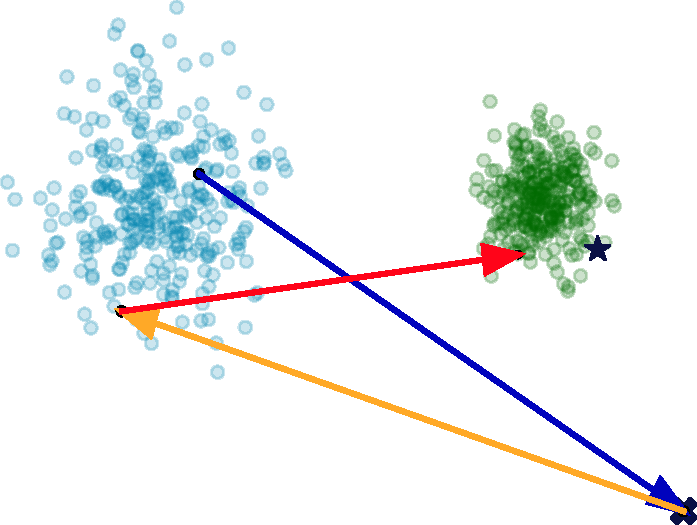
\includegraphics[width=\textwidth]{figures/toy/final_0.00_toy.pdf} % Replace 'figure1.png' with your first figure
    \caption{t = 0}
        \label{fig:figure1}
    \end{subfigure}%
    \hfill % Add horizontal space between figures
    \begin{subfigure}{0.3\textwidth}
        \centering
    \includegraphics[width=\textwidth]{figures/toy/final_0.56_toy.pdf} % 
     \caption{t = 0.56}
        \label{fig:figure2}
    \end{subfigure}%
    \hfill 
    \begin{subfigure}{0.3\textwidth}
        \centering
    \includegraphics[width=\textwidth]{figures/toy/final_0.89_toy.pdf} 
    \caption{t = 0.89}
        \label{fig:figure3}
    \end{subfigure}

    \caption{Our method on a 2D denoising task ($\sigma=1.5$) with Gaussian distributions. 
    An OT Flow Matching model is trained to sample from $P_1 = \mathcal N(m, s^2 \Id)$, with $m=7$ and $s=0.5$.
    At each time step, it performs a standard gradient step on the datafit, followed by a projection onto flow trajectories at time $t$, and finally applies the time-dependent denoiser $D_t$.}
    \label{fig:2DEX_gaussian_to_gaussian}
\end{figure}


%
%-----------------------------------------------
\section{Background}
%-----------------------------------------------
% As our method, PnP-Flow, leverages the Plug-and-Play algorithmic scheme while using a generative Flow Matching model, we next provide some useful insights on both frameworks.
We next provide background on both Plug-and-Play algorithms and Flow Matching models.
%-----------------------------------------------
\subsection{Plug and Play}
%-----------------------------------------------
PnP algorithms were introduced as extensions of proximal splitting methods like Forward-Backward Splitting (FBS) or the alternating direction method of multipliers (ADMM). These are first-order optimization algorithms for solving problem \eqref{eq:min_pb_regularized}, alternating between a proximal step on the regularization and a gradient and/or proximal step on the data-fidelity function. 
The proximal operator $\prox_{\gamma R}: \R^d \to \R^d$, $\gamma >0$ is defined by $\prox_{\gamma R} (y) \coloneqq \argmin_{x \in \R^d} \left\{\frac12 \| y-x\|^2 + \gamma R(x) \right\}$.
In this paper, we assume that the data-fidelity $F$ is differentiable with Lipschitz continuous gradient and we focus on the FBS algorithm, corresponding to Algorithm~\ref{alg:FBS}.
The convergence of FBS to a minimizer of $F+R$ is guaranteed as long as the stepsize is chosen as $\gamma \in (0,1/\text{Lip} (\nabla F))$, where $\text{Lip} (\nabla F)$ is the Lipschitz constant of $\nabla F$ \citep{combettes2005signal}.

\begin{minipage}{0.48\textwidth}
\RestyleAlgo{ruled}
\begin{algorithm}[H]
\textbf{Initialization:}  $x^{(0)} \in \mathbb{R}^d$, $\gamma > 0$\\
% \textbf{Iterations:}  \\
 \For{$r = 0, 1, \ldots$}
 {
$z^{(r+1)} = x^{(r)} - \gamma \nabla F(x^{(r)})$ \\
$x^{(r+1)} = \prox_{\gamma R}(z^{(r+1)}) $ \
}
\caption{FBS}
\label{alg:FBS}
\end{algorithm}
\vspace{0mm}
\end{minipage}
\hfill
\begin{minipage}{0.48\textwidth}
\RestyleAlgo{ruled}
\begin{algorithm}[H]
 \textbf{Initialization:} $x^{(0)} \in \mathbb{R}^d$, $\gamma > 0$ \\
 % \textbf{Iterations:} \\
 \For {$r = 0, 1, \ldots$}{
$ z^{(r+1)} = x^{(r)} - \gamma \nabla F(x^{(r)}) $ \\
$ x^{(r+1)} = D (z^{(r+1)}) $ \algorithmiccomment{PnP step}
}
\caption{ PnP-FBS }
\label{alg:PNP-FBS}
\end{algorithm}
\vspace{0mm}
\end{minipage}

Observing that computing $\prox_{\gamma R}$ corresponds to solving a Gaussian denoising problem with regularization $\gamma R$, \citet{venkatakrishnan13pnp} proposed to replace it with an \emph{off-the-shelf} denoiser $D: \R^d \longrightarrow \R^d$, which can be independently designed or learned (see Algorithm~\ref{alg:PNP-FBS}).

Many PnP-FBS methods, such as \cite{meinhardt17learnprox,zhang2017beyond, zhang2021plug, SWK2019, terris20firmly, HNS2021, hurault2022gradient, tan2024provably} use neural network denoisers. 
Most of these PnP-FBS algorithms do not converge \citep{zhang2017beyond, SKM2019} and convergence guarantees usually assume non-expansiveness of the denoiser \citep{pesquet2021learning,ryu19prox, hurault2022prox}. 
% For instance, we do not have convergence if we use  the DnCNN denoiser \citep{zhang2017beyond, SKM2019}.
% Convergence guarantees for PnP-FBS require non-expansiveness of the denoiser. 
% Various strategies exist to build PnP algorithms with are provably convergent \citep{ryu19prox,HNS2021,pesquet2021learning,terris20firmly,hurault2022gradient,hurault2022prox,tan2024provably}. 
Yet, constraining the Lipschitz constant of a neural network, e.g., through weight clipping, spectral normalization or averaged operator constructions harms in general its expressiveness \citep{ryu19prox}.

% In this paper, we propose to use a time dependent denoiser based on a learned velocity field via Flow Matching. 

%-----------------------------------------------------------------
\subsection{Flow Matching}
%-----------------------------------------------------------------
\label{subsection:flow_matching}
Let $\mathcal P_2(\R^d)$ denote the subspace of probability measures on $\R^d$ having a finite second moment. Let $P_0$ denote the latent probability measure and $P_1$ the target probability measure (i.e., the data distribution). We denote $\cdot_\sharp$ the push-forward operation. We denote $\Gamma(P_0,P_1)$ the
set of couplings $\pi \in \mathcal P(\R^d \times \R^d)$ 
having marginals $P_i \in \mathcal P_2(\R^d)$, $i=0,1$, and $\Gamma_{\text{o}}(P_0,P_1)$ the set of optimal couplings minimizing the Wasserstein-2 distance \citep{villani}. We now start with any coupling $\pi \in \Gamma(P_0,P_1)$. 
% For this subsection, we mainly follow \citep{ambrosio2008}.

% The Wasserstein(-2) metric is defined by
% \begin{align} \label{wasserstein}
% W^2_2(P_0, P_1)
% \coloneqq 
% \min_{\pi \in\Gamma(P_0,P_1)} \int_{\R^d \times \R^d}\|x-y\|^2 \, \dd \pi(x,y)
% =
% \min_{(X_0,X_1) \sim \pi\in\Gamma(P_0,P_1) } \E\left[ \|X_0-X_1\|^2 \right],
% \end{align}
% where $\Gamma(P_0,P_1)$ denotes the
% set of couplings/plans $\pi \in \mathcal P(\R^d \times \R^d)$ 
% having marginals $P_i \in \mathcal P_2(\R^d)$, $i=0,1$. Together with the Wasserstein metric, $\mathcal P_2(\R^d)$
% is a complete metric space.
% The set of minimizers of \eqref{wasserstein} are the optimal couplings
% $\Gamma_{\text{o}}(P_0,P_1)$.
% In this paper, we restrict ourselves to absolutely continuous measures with respect to the Lebesgue measure and address measures also by their densities. In this case, by Brenier's theorem \citep{villani, brenier1991}, there is a unique optimal plan $\pi \in \Gamma(P_0,P_1)$ which minimizes \eqref{wasserstein} and it is
% induced by a unique (Borel) measurable optimal transport map $T\colon \R^d \to \R^d$ called Monge map, 
% which minimizes
% \begin{equation} \label{eq:monge}
% 	 W_2^2(P_0, P_1) =
%  \min_{T\colon  \R^d \to  \R^d}  
%   \int_{\R^d}  \|x - T(x) \|_2^2  \, \dd P_0(x)
%     \quad \text{subject \; to} \quad T_\sharp P_0 = P_1,
%   \end{equation}
% i.e.,
% $\pi = ({\rm{Id}}, T)_\sharp P_0 \coloneqq P_0\circ ({\rm{Id}}, T)^{-1}$. 

% In complete metric spaces, we can consider absolutely continuous curves depending on the metric of the space.
% In the Wasserstein space, 
% a weakly continuous curve $P: [0,1] \to \mathcal P_2(\R^d)$, $t\mapsto P_t$ is said to be \emph{absolutely continuous} if there exists a Borel vector field 
% $
% v:[0,1]\times \R^d\to\R^d$ 
% with 
% $
% \int_0^1 \| v_t \|_{L_2(\R^d,P_t)} \, \dd t < \infty
% $ 
% such the curve satisfies the \emph{continuity equation} 
% \begin{equation}\label{eq:continuity}\tag{\text{CE}}
% \partial_t P_t +  \nabla\cdot(P_t v_t) = 0
% \end{equation}
% in the sense of distributions,
% (see, e.g., \citep{ambrosio2008}). For such an absolutely continuous curve
% $P_t$ with vector field $v_t$ fulfilling a mild additional condition, there exists a solution 
% $f:\R^d \times [0,1] \to \R^d$ of the ODE
% \begin{align}\label{eq:flow_ode}
% \partial_t f(t,x)=v(t, f(t,x)), \quad f(0,x)=x
% \end{align}
% such that $P_t = f(\cdot,t)_\sharp P_0$.

% The main idea behind Flow Matching is to consider the specific absolutely continuous curve $P_t \coloneqq (e_t)_\sharp \pi$
% defined by random variables with corresponding laws as
% \begin{equation} \label{fm}
% X_t = (1-t) X_0 + t X_1, \quad P_t \coloneqq (e_t)_\sharp \pi.
% \end{equation}
% with $e_t(x, y):= (1-t)x + ty$. Then, there is specific velocity field $v$ such that $(P_t, v_t)$ satisfies the continuity equation \eqref{eq:continuity}.
% The couplings $\pi$ are usually chosen as independent coupling $\pi = P_0 \times P_1$ (\citep{lipman2023flow}) or as OT coupling $\pi \in \Gamma_{\text{o}}(P_0,P_1)$ (\citep{liu2022rectified}).
The core idea behind Flow Matching is to define a specific target probability path $t \mapsto P_t$, $t \in [0,1]$, between $P_0$ and $P_1$. Let $P_t \coloneqq (e_t)_\sharp \pi$, where the map $e_t(x_0, x_1) := (1-t)x_0 + tx_1$ interpolates between (a latent sample) $x_0$ and (a data sample) $x_1$.
% {\color{red} Never let two formulas meet each other}
The path $P_t$ can be shown to be an absolutely continuous curve, so there exists a Borel vector field 
$v:[0,1]\times \R^d\to\R^d$ 
% with 
% $\int_0^1 \| v_t \|_{L_2(\R^d,P_t)} \, \dd t < \infty$ 
such that the curve satisfies the \emph{continuity equation} 
\begin{equation}\label{eq:continuity}\tag{\text{CE}}
\partial_t P_t +  \nabla\cdot(P_t v_t) = 0
\end{equation}
in the sense of distributions \citep{ambrosio2008}. 
% {\color{red} no brackets are necessary for see; further this is only half of the definition of an absolutely cont. curve}
In addition, there exists a solution 
$f:[0,1] \times \R^d \to \R^d$ of the ODE
\begin{align}\label{eq:flow_ode}
\partial_t f(t,x)=v_t(f(t,x)), \quad f(0,x)=x
\end{align}
such that $P_t = f(t, \cdot)_\sharp P_0$. If $f$ is known, then a sample $x_1$ from the target distribution $P_1$ can be drawn by first sampling $x_0 \sim P_0$ and then defining $x_1 = f(1, x_0)$.


The goal of Flow Matching is to learn the velocity field of the flow ODE \eqref{eq:flow_ode}. This learning process consists in minimizing the loss function
\begin{align}\label{fm}
    \mathcal{L}_{\text{FM}}(\theta) :=\E_{t\sim \mathcal U [0,1],x\sim P_t}\left[\|v^\theta_t(x)-v_t(x)\|^2\right],
\end{align}
where $v^\theta$ is parametrized by a neural network with weights $\theta$.
Unfortunately, in practice, the true velocity field $v_t(x)$ is not available.
However,
\citet{lipman2023flow} showed that
% \textcolor{blue}{GABI: then skip the blue part it makes things not better :showed that for a particular choice of velocity field satisfying \eqref{eq:continuity}}, 
minimizing $\mathcal{L}_{\text{FM}}(\theta) $ is equivalent to minimizing the Conditional Flow Matching (CFM) loss:  $\mathcal{L}_{\text{CFM}}(\theta)  = \mathcal{L}_{\text{FM}}(\theta) + \text{const}$, where
\begin{align} \label{cfm}
\mathcal{L}_{\text{CFM}}(\theta):=\E_{t\sim \mathcal U [0,1],(x_0,x_1)\sim\pi}\left[\|v^\theta_t \left(e_t(x_0, x_1)\right)-(x_1-x_0)\|^2\right] .
\end{align} 
Minimizing this loss only requires sampling from the coupling $\pi$. For example, if $\pi = P_0 \times P_1$ is the independent coupling, we only need samples from the latent and target distributions. If instead, $\pi \in \Gamma_{\text{o}}(P_0, P_1)$ is an optimal coupling, then we can use a standard optimal transport solver to (approximately) sample from $\pi$, as proposed in \citet{pooladian2023multisample, tong2024improving}. 



\paragraph{Straight-line flows}
% \begin{remark}[Straight-line flows] \label{rem:straight_line}
Let $v\colon [0,1] \times \R^d \longrightarrow \R$ and let $f$ be a solution to the flow ODE associated with $v$.
Given $(X_0,X_1) \sim \pi$, we call $(f,v)$
% a solution to the flow ODE $f(t,x) = \int_0^t  v_s(f(s,x)) ds + x$  
a \emph{straight-line Flow Matching pair} connecting $X_0$ and $X_1$ if $X_t = f(t,X_0)$ almost surely, where $X_t$ is defined as $X_t:= e_t((X_0,X_1)) = t X_1 + (1-t)X_0$ \citep{liu2023flow, pooladian2023multisample}. Note that this directly implies $v_t(f(t,X_0)) = \partial_t f(t,X_0)  = \partial_t X_t = X_1-X_0$ almost surely.

We will focus on such straight-line flows later in the paper. Straight or nearly straight paths are preferred since they represent the shortest distance between two points and can be simulated with fewer steps of an ODE solver. This has been explored in many recent works that want to speed up sampling, such as \citet{kornilov2024optimal, pmlr-v202-lee23j, yang2024consistencyflowmatchingdefining}.  A particular case of straight-line pair is given by OT couplings \citep{pooladian2023multisample, tong2024improving}. Indeed, for $\pi \in \Gamma_{\text{o}}(P_0, P_1)$ with Monge map $T: \R^d \to \R^d$ such that $X_1=T(X_0)$, there exists a velocity field $v$ for which the pair $(P_t, v_t)$ is a solution of the continuity equation \eqref{eq:continuity}, and such that for all $x \in \R^d$
\begin{equation} \label{eq:velocity_OT}
    v_t (f(t, x)) = T(x) - x,
\end{equation}
where $f$ is the solution of the ODE \eqref{eq:flow_ode}, see \citet{ambrosio2008, pooladian2023multisample, CHSW2024} for the precise conditions. By integrating \eqref{eq:velocity_OT}, it is clear that $(f, v)$ is a straight-line Flow Matching for the coupling $(X_0, T(X_0))$, since $X_t = (1-t)X_0 + tX_1 = (1-t)X_0 + tT(X_0) = X_0 + \int_0^t v_s(f(s,X_0)) ds = f(t,X_0)$.
% \end{remark}



%-----------------------------------------------
\section{PnP meets Flow Matching}
%-----------------------------------------------
\subsection{Denoising Operator from Flow Matching}
% \begin{wrapfigure}[13]{r}{0.4\textwidth} 
%     \centering
%     \includegraphics[width=\linewidth]{figures/sketch_OT_EX.pdf} 
%     \caption{The PnP operator $D_t$ for optimal OT Flow Matching.}
%     \label{fig:OTEX_Denoiser}
% \end{wrapfigure}
Let $X_0 \sim P_0$ and $X_1 \sim P_1$ with joint distribution $(X_0, X_1) \sim \pi$. Assume we have access to a pre-trained velocity field $v^\theta$. Then we define, for $t\in [0,1]$, the following time-dependent denoiser
\begin{equation} \label{eq:denoiser}
    D_t  \coloneqq \Id + (1-t) v^\theta_t,
\end{equation}
and we propose to use it within a PnP framework. 

To motivate the choice of the denoiser in \eqref{eq:denoiser}, recall  that for a fixed time $t \in [0, 1]$, the minimizer $v_t^*$ of the CFM loss \eqref{cfm} over all possible vector fields reads 
\begin{equation}
    v_t^* (x) = \mathbb{E}[X_1 - X_0|X_t = x],
\end{equation}
where $X_t := e_t(X_0, X_1) = (1-t) X_0 + t X_1$ \citep{benton2024error,liu2023flow}. Assume we are in the ideal case where $v_t^\theta= v_t^*$.
%
% \color{blue} The Conditional Flow Matching loss is a Minimum Squared Error (\citep{benton2024error,liu2023flow}), whose minimum $v_t^*$ (for a fixed time $t \in [0, 1]$) is the conditional expectation $v_t^* (x) = \mathbb{E}[X_1 - X_0|X_t = x]$ where $X_t := e_t(X_0, X_1) = (1-t) X_0 + t X_1$.
Then it follows that, for any $x \in \R^d$ and $t \in [0,1]$,
\begin{align}
      D_t (x) & = x + (1-t) v^*_t(x)  \label{helper}\\
      & = \mathbb E_{(X_0, X_1) \sim \pi} \left[ X_t + (1-t) (X_1 - X_0) | X_t = x\right] \nonumber \\
      & = \mathbb E_{(X_0, X_1) \sim \pi} \left[ X_1 | X_t = x \right] .
\end{align}
% Theoretically, we see that
% \begin{align}
%       D_t (X_t) & = X_t + (1-t) v^*_t(X_t)  \label{helper}\\
%       & = \mathbb E_{(X_0, X_1) \sim \pi} \left[ X_t + (1-t) (X_1 - X_0) | X_t \right] \nonumber \\
%       & = \mathbb E_{(X_0, X_1) \sim \pi} \left[ X_1 | X_t \right] .
% \end{align}
Hence, the operator $D_t$ can be understood at the best approximation of $X_1$ given the knowledge of $X_t$, which is also used in \citet{pokle2024trainingfree} and  \citet{zhang2024flow}. 
% The operator is visualized in Fig.~\ref{fig:OTEX_Denoiser}, where one can see that the operator maps points in the direction of $X_1$.
% with a length that respects the straight paths. 
\color{black}
%

Just as standard PnP denoisers minimize the MSE loss between noisy and clean samples, the operator $D_t$ is the minimizer of $L^2$-problem $\min_{g} \E_{(X_0, X_1) \sim \pi} [||X_1 -g(X_t)||^2]$, projecting any noisy point taken along the path onto the target distribution. 
In particular, the following proposition holds, demonstrating that the best denoising performance is achieved with straight-line flows.
% In particular, by the following proposition, the loss $\E_{(X_0, X_1) \sim \pi} [||X_1 -D_t(X_t)||^2]$
% % our denoiser $D_t(x) = \mathbb{E}[X_1|X_t = x]$ 
% is zero for all $t \in (0,1)$, if and only if the corresponding velocity field follows a straight path, which is similar to the proof idea used in \citep{pmlr-v202-lee23j}.
%
\begin{proposition}\label{prop:straight}
Assume $v:=v^\theta$ is continuous and assume that, given $v$, the Flow ODE \eqref{eq:flow_ode} has a unique solution $f$.
Then the denoising loss $\mathbb{E}_{(X_0,X_1) \sim \pi}[\Vert D_t(X_t) -X_1 \Vert^2]$ is equal to 0 for all $t \in [0,1]$, if and only if the couple $(f, v)$ is a straight-line Flow Matching pair between $X_0$ and $X_1$.
\end{proposition}

The proof can be found in Appendix~\ref{sec:app_proof_straight}.

As stated in Section~\ref{subsection:flow_matching}, a special case of straight-line flows is given by OT Flow Matching for which we recover $D_t(X_t) = X_1$. Indeed, in this case, $D_t$ reduces to $T(X_0) = X_1$, with $T$ the Monge map between $P_0$ and $P_1$.
% {\color{blue} The connection to straight-line flow pairs can even be improved in the case of OT Flow Matching.
% %
% \paragraph*{Denoiser from OT Flow Matching} One special case of straight line Flow Matchings is the OT Flow Matching framework, where we consider $\pi \in \Gamma_{\text{o}} (P_0,P_1)$ with corresponding Monge map $T$. Then, using Equation \eqref{eq:velocity_OT}, we obtain
% \begin{align*}
% D_t(f(t,x)) &= f(t,x) + (1-t) v_t \left(f(t,x) \right) 
% = (1-t) x + t T(x) + (1-t)(T(x) - x) 
% = T(x).
% \end{align*}
% Hence $D_t$ maps any noisy input $x_t$ taken along the path, i.e., any point on $f(t,x)$ for $x \in \R^d$, to a clean image $T(x)$ from the distribution of $X_1$.}
%
%
% Through the following remark, we emphasize that our denoiser was specifically designed for Flow Matching generative models, inspired by the intuition of straight paths discussed earlier.
We next discuss whether diffusion models induce straight-line flows.

\begin{remark}[Flow Matching versus diffusion models]
Contrary to OT Flow Matching, diffusion models, which are also flow ODE methods, do not generally induce straight paths. Indeed, during diffusion training, the target probability path takes the form $\tilde{X}_t = \alpha_t X_0 + \beta_t X_1$ with $\alpha_t \in (0,1)$ and $\beta_t =\sqrt{1-\alpha_t^2}$ \citep{song2021scorebased, liu2023flow}, which clearly does not match the desired straight path $X_t = (1-t)X_0 + tX_1$. The non-straightness of the flow generated by diffusion models is illustrated in \citet[Figure 5]{liu2023flow,liu2022Ot}. On the other hand, a non-straight path obtained with Flow Matching (for instance, using an independent coupling $\pi$) can be \emph{rectified} to a straighter one following the procedure described in \citet{liu2023flow}.
\end{remark}
%-------------------------------------------------
\subsection{PnP Flow Matching Algorithm}
%-------------------------------------------------------
% \begin{wrapfigure}[14]{r}{0.4\textwidth} 
%     \centering
%     \includegraphics[width=\linewidth]{figures/interpolation_step.pdf} 
%     \caption{The PnP operator $D_t$ for optimal OT Flow Matching.}
%     \label{fig:OTEX_Interpolation}
% \end{wrapfigure}
In the previous section, we built a denoiser $D_t$ (defined in \eqref{eq:denoiser}). We now want to plug it in a Forward-Backward Splitting algorithm in order to solve inverse problems. 
% Yet, our PnP denoiser $D_t$ in \eqref{eq:denoiser} 
% differs from classical PnP operators
% by two key features:
% first, $D_t$ is time-dependent, which means that the iterations of the PnP algorithm must also be time-dependent.
% Second, the operator $D_t$ maps noisy images towards images from the target distribution only when the inputs are sampled along the path $X_t = (1-t) X_0 + t X_{1}$. 
% In other words, the desired regularizing behavior of $D_t$ is guaranteed only for inputs that lie along this path at time $t$.
% Since the output of the gradient step has no reason to belong to an existing trajectory along this path, we propose an intermediate reprojection step that maps the output of the gradient step back to a noisy image located on a path from $X_0$ to $X_1$ at time $t$.
% More precisely, at each time $t \in [0,1]$, given the current iterate,
% %$x_t$
% our algorithm does the following updates:
Yet, our algorithm differs from the classical PnP-FBS (Algorithm~\ref{alg:PNP-FBS}) in two key aspects.
First, the iterations of the our algorithm depend on time because of the definition of $D_t$.
Second, we introduce an intermediate reprojection step between the gradient step on the data-fidelity term and the denoising step.
More precisely, at each time $t \in [0,1]$, given the current iterate $x$,
our algorithm does the following updates:
\begin{wrapfigure}[19]{r}{0.35\textwidth} 
    \centering
    \vspace{1.6cm}
    \includegraphics[width=4.5cm]{figures/interpolationstep.pdf} 
    \caption{Illustration of the interpolation step. \label{fig:OTEX_Interpolation}}
\end{wrapfigure}

\begin{enumerate}
    % \begin{minipage}[l]{0.52\textwidth} 
    \item \textbf{Gradient step:} a gradient step on the data-fidelity term, mapping $x$ to $z= x- \gamma \nabla F(x)$ for a given learning rate $\gamma >0$.
    % where one defines $z_t = x_t - \gamma_t \nabla f(x_t)$ 
       % Except for the first step, this step is done after the PnP denoising step, which denoises an image towards one from $P_1$. 
    % However, the subsequent PnP denoiser $D_t$ requires samples from the measure $P_t$.
    %Therefore, to 'reproject' along the paths of $X_t$,
    \item \textbf{Interpolation step:} 
     In a standard Forward-Backward scheme, the denoiser operator is applied right after the gradient step.
     Yet, as discussed earlier, our operator $D_t$ was specifically designed to correctly denoise inputs drawn from the straight path $X_t = (1-t) X_0 + t X_1$.
    If the output $z$ from the gradient step  at time $t$ does not lie in the support of $X_t$, there is a high chance that the denoising will not be effective,
     hence the need to ``reproject'' 
     it along the flow paths before applying $D_t$.
     To achieve this, we perform a linear interpolation on $z$, as illustrated in Figure~\ref{fig:OTEX_Interpolation}: at time $t$, we define $\tilde{z} = (1-t)\varepsilon + t z$, where $\varepsilon$ is a noise sample drawn from $P_0$. Note that while $\varepsilon$ is sampled from $P_0$, it is not necessarily coupled to $z \sim P_1$ via $\pi$. If it were, $D_t$ would map $\tilde{z}$ directly back to $z$, annihilating the denoising effect. 
     % Drawing $\varepsilon$ independently from the gradient step's output $z$ benefits the algorithm by allowing it to deviate from a straight trajectory.

     
     % We justify this reprojection strategy reasoning by 'induction':
    % \end{minipage}
    % \hfill
    
%     \begin{figure}
%      \begin{minipage}[r]{0.3\textwidth}
%     \includegraphics[width=\textwidth]{figures/interpolation_step.pdf} 
% \end{minipage}
%  \caption{Illustration of the interpolation step. \label{fig:OTEX_Interpolation}}
% \end{figure}



     % \begin{itemize}
     %     \item[--] at time $t =0$, $D_0$ is fed with $\epsilon \sim P_0$, a realization of $X_0$.
     %     \item[--] at time $t >0$, what goes into the gradient step must be within (or not far from) the image space as it is the output of the previous denoising step. Choosing the stepsize $\gamma_t$ small enough can ensure the output of the gradient step also remains within the image space, in which case, the linear interpolation indeed gives a realization of $X_t$, as desired. 
     % \end{itemize} 
     % As discussed earlier, the denoiser $D_t$ was specifically designed to correctly denoise inputs $x_t$ drawn from the straight path $X_t = (1-t)X_0 + t X_1$. However, if the output $z_t$ from the gradient step does not lie on the support of $X_t$, there is a high chance that the denoising will not be effective, and the output of the denoiser could become unpredictable in this case. Therefore, prior to the denoising step, we need to 'reproject' $z_t$ along the flow paths. To achieve this, we perform a linear interpolation, mapping $z_t$ to $\tilde{z}_t = (1-t)\varepsilon + t z_t$, where $\varepsilon$ is a noise sample drawn from $P_0$. Then $\tilde{z}_t$ can be interpreted as a realization of the random variable $X_t$ and we justify it as follows. The key idea is that, by induction, $z_t$ remains within the image distribution space because $x_t$ does. At $t=0$, $\tilde{z}_0$ is sampled from $X_0$, ensuring that after a small time step $\Delta_t$, the update $x_{\Delta_t}$ remains in the image space. Assuming that at time $t-\Delta_t$, $x_{t-\Delta_t}$ is within the image space, then, given a sufficiently small learning rate, $z_t$ will also remain within the image space. 

     % This linear interpolation can also be understood as a way to give at time $t$ to the pre-trained model $v_\theta( \cdot, t)$ with an image that resembles what it has seen during the training.
\item \textbf{PnP Denoising step}: the operator $D_t$ is applied to the output $\tilde{z}$ of the interpolation step, regularizing the current image by pushing it towards the distribution of $X_1$. 
%{\color{blue} Note that, to obtain a deterministic output at each time $t$ of the %algorithm, one can take the expectation of $D_t(\tilde{z}(\varepsilon))$ with respect %to $\varepsilon \sim P_0$.}
\end{enumerate}
\
The resulting discrete-time algorithm is given in Algorithm \ref{algo:pnp_flow}. Figure \ref{fig:2DEX_gaussian_to_gaussian}  illustrates the three steps of the algorithm on a denoising problem with a Gaussian prior. 
%
\begin{center}
\RestyleAlgo{ruled}
\begin{algorithm} 
\textbf{Input:} Pre-trained network $v^\theta$ by Flow Matching, time sequence $(t_n)_n$ either finite with $t_n= n/N$, $N \in \N$ or infinite with $\lim_{n \rightarrow +\infty} t_n = 1$, adaptive stepsizes $(\gamma_n)_n$.\\
\textbf{Initialize:} $x_{0} \in \R^d$.\\
\For{$n = 0, 1, \dots,$}
{
   $z_{n} = x_{n}-  \gamma_{n} \nabla F( x_{n}) $. \algorithmiccomment{Gradient step on the data-fidelity term} \\
   $\tilde z_{n} = (1-t_n)  \varepsilon +  t_n z_n $, \,$\varepsilon \sim P_0$ \quad \algorithmiccomment{Linear interpolation} \\
   $x_{n+1} = D_{t_n} (\tilde{z}_n) $ \algorithmiccomment{PnP step with denoiser \eqref{eq:denoiser}} \\
}
\Return $x_{n+1}$
\caption{PnP Flow Matching\label{algo:pnp_flow}}
\end{algorithm}
\end{center}
%---------------------------------------------------
\vspace{-0.8cm}
\begin{remark}[Averaging in the denoising step]
Instead of drawing one noise realization, we can also average over multiple samples $\varepsilon \sim P_0$ in the last step of the algorithm:
$x_{n+1} \coloneqq \E_{\varepsilon \sim P_0}[D_{t_n} (\tilde{z}_n(\varepsilon))]$ with $\tilde z_{n}(\varepsilon) \coloneqq (1-t_n)  \varepsilon +  t_n z_n $.
The algorithm's output is then deterministic. In practice, averaging over a few realizations slightly improves the numerical results.
\end{remark}

\paragraph{Time dependent learning rate} Using a constant learning rate independent of time can give too much importance to the data fit.  
For example, if $\gamma_t = 1$ for all $t \in [0,1]$ on a simple denoising task, the algorithm will return the noisy sample $y$ since $D_1 = \rm{Id}$. To prevent this, $\gamma_t$ should decrease with $t$ to balance the contributions of the datafit and the denoiser. We set $\gamma_t = (1-t)^\alpha$ with $\alpha \in (0,1]$ for the remainder of the paper. This choice yields good numerical results in our experiments, but alternative values for $\gamma_t$ could also be explored.

\paragraph{Convergence}
Assuming that the sequence produced by the algorithm is bounded in the infinite time regime, we have the following convergence result.
\begin{proposition}\label{prop:convergence}
Assume that $F: \R^d \to \R$ is continuously differentiable
and that the learned vector field $v: [0,1] \times \R^d  \rightarrow \R^d$
is continuous.
Let the time sequence $(t_n)_{n \in \N}$ satisfy $\sum_{n=0}^\infty (1-t_n) < +\infty $ and let $\gamma_n \coloneqq 1-t_n$, $n \in \N$. 
If the sequence $(x_n)_{n\in \N}$  obtained by Algorithm \ref{algo:pnp_flow} is bounded, then it converges.
\end{proposition}
The proof can be found in Appendix \ref{sec:app_proof}.

% \begin{proposition}
% Let the time sequence $(t_n)_{n \in \N}$ be a geometric sequence of the form $t_n =1-\beta^n$ for $\beta \in (0,1)$ and the learning rate sequence $(\gamma_n)_{n \in \N}$ be constant equal to $\gamma >0$. Let $(x_n)_{n\in \N}$ be the sequence obtained with Algorithm \ref{algo:pnp_flow}. Assume:
% \begin{itemize}
% \item $\epsilon =0$ in the interpolation step in the algorithm,
% \item $(x_n)_{n \in \N}$ is bounded by a constant $C$,
% \item $f$ is convex and differentiable, and $\nabla f$ is $L_f$-Lipschitz,
% \item $v$ is continuous on $\R^d \times [0,1]$.
% \end{itemize} Then $\Vert x_{n+1} - x_n \Vert \underset{n \rightarrow +\infty}{\longrightarrow} 0$. Moreover, the following convergence rate holds:
% \begin{equation}
%     \Vert x_{n+1} - x_n \Vert \leq \beta^n(1-\beta) + \exp\left\{\frac{ L_v (1 + \gamma L_f)\beta^{n-1}}{1-\beta} (\beta^2 - 1) \right\} \exp\left\{\frac{ L_v (1 + \gamma L_f)}{1-\beta} \right\} \beta^{n},
% \end{equation}
% where $L_v$ is a constant such that $\Vert v(z_1, t_1) - v(z_2, t_2)\Vert \leq L_v \left( \Vert z_1 - z_2 \Vert + | t_1 - t_2 |\right)$ for any $z_1, z_2 \in \mathcal{K}$, where $\mathcal{K}:= \{x - \gamma \nabla f(x),\; x \in \mathcal{B}(0, C) \}$.
% \end{proposition}

% \begin{proof}
% Let $n \in \N$ and $z_n := t_n(x_n - \gamma \nabla f(x_n))$. We denote $v_n = v(z_n, t_n)$, so that $x_{n+1} = z_n + (1-t_n) v( z_n, t_n)$
% \begin{align}\label{eq:decomp_diff}
%     \Vert x_{n+2} - x_{n+1} \Vert &\leq \Vert z_{n+1} -  z_{n} \Vert + \Vert (1-t_{n+1})v_{n+1}- (1-t_{n})v_{n}\Vert.
% \end{align}
% We now upper-bound each term on the right-hand side. For the first term, it holds that
% \begin{align}
%      \Vert z_{n+1} -z_{n} \Vert &\leq |t_{n+1}| \Vert x_{n+1} - \gamma \nabla f(x_{n+1}) - x_n + \gamma \nabla f(x_{n}) \Vert + \Delta_n \Vert x_n -\gamma \nabla f(x_{n}) \Vert \nonumber \\
%      &\leq  |t_{n+1}| \Vert x_{n+1} - \gamma \nabla f(x_{n+1}) - x_n + \gamma \nabla f(x_{n}) \Vert + \Delta_n M_1,
%     \end{align}
% where $\Delta_n := t_n - t_{n+1}$ and $M_1 > 0$ is a constant such that $\Vert x_n -\gamma \nabla f(x_{n}) \Vert \leq M_1$. 
% % In addition, 
% % \begin{align}
% % \Vert x_{n+1} - \gamma \nabla f(x_{n+1}) - x_n + \gamma \nabla f(x_{n}) \Vert^2 &= \Vert x_{n+1} - x_{n}\Vert^2 - 2\gamma \langle x_{n+1} - x_{n}, \nabla f(x_{n+1}) - \nabla f(x_{n}) \rangle \nonumber \\ &+ \gamma^2 \Vert \nabla f(x_{n+1}) - \nabla f(x_{n})\Vert^2 
% % \end{align}
% In addition, 
% \begin{align}
% \Vert x_{n+1} - \gamma \nabla f(x_{n+1}) - x_n + \gamma \nabla f(x_{n}) \Vert &\leq \Vert x_{n+1} - x_{n}\Vert + \Vert \gamma_{n+1} \nabla f(x_{n+1}) - \gamma_{n}\nabla f(x_{n})\Vert , 
% \end{align}
% and since $\nabla f$ is $L_f$-Lipschitz
% \begin{align}
%     \Vert \gamma_{n+1} \nabla f(x_{n+1}) - \gamma_{n}\nabla f(x_{n})\Vert 
% &\leq |\gamma_n - \gamma_{n+1} | \Vert \nabla f(x_{n+1})\Vert + \gamma_n \Vert \nabla f(x_{n+1}) - \nabla f(x_{n}) \Vert \nonumber \\ &\leq \Delta_n M_2 + \gamma_n L_f \Vert x_{n+1} - x_{n}\Vert,
% \end{align}
% with $M_2 >0$ is such that $\Vert \nabla f(x_{n}) \Vert  \leq M_2$ for all $n \in \N$.
% Thus
% \begin{align}
%      \Vert z_{n+1} -z_{n} \Vert &\leq  t_{n+1} (1+ L_f\gamma_n) \Vert x_{n+1} - x_{n}\Vert + \Delta_n (M_1 + t_{n+1} M_2).\label{eq:bound_term_1}
% \end{align}
% For the second term in \eqref{eq:decomp_diff}, we have:
% \begin{align}
%     \Vert (1-t_{n+1})v_{n+1}- (1-t_{n})v_{n}\Vert & \leq (1-t_{n+1}) \Vert v_{n+1} - v_{n} \Vert + \Delta_n \Vert v_n \Vert \nonumber \\
%     &\leq (1-t_{n+1}) L_v (\Vert z_{n+1} -z_{n} \Vert+ \Delta_n) +  \Delta_n M_3, \label{eq:bound_term_2}
% \end{align}
% where $M_3 >0$ is such that $\Vert v_n \Vert  \leq M_3$. Hence, combining \eqref{eq:bound_term_1} and \eqref{eq:bound_term_2}, 
% \begin{align}
%      \Vert x_{n+2} - x_{n+1} \Vert & \leq  t_{n+1} (1+ L_f\gamma_n)\Vert x_{n+1} - x_{n}\Vert + \Delta_n (M_1+t_{n+1} M_2)  \nonumber \\  & \qquad + (1-t_{n+1}) L_v (\Vert z_{n+1} -z_{n} \Vert+ \Delta_n)+  \Delta_n M_3 \nonumber\\
%      & \leq \Vert x_{n+1} - x_{n}\Vert |t_{n+1}| (1+ L_f\gamma_n) 
%  \left( 1+ (1-t_{n+1}) L_v\right) \nonumber \\  & \qquad + \Delta_n \left(M_1 + t_{n+1} M_2+ (1-t_{n+1}) L_v  M_1 + 1 +   M_3 \right) \label{eq:majoration_diff}
% \end{align}
% Using the expression of $t_n$ and $\gamma_n$, \eqref{eq:majoration_diff} rewrites
% \begin{equation}
%     \Vert x_{n+2} - x_{n+1} \Vert  \leq (1 + a_n) \Vert x_{n+1} - x_{n}\Vert + b_n,
% \end{equation}
% where for all $n \in \N$, $a_n = \beta^n (-\beta + L_v \beta - L_v \beta^{n+1}+ L_f -L_f \beta^{n+1} + L_v L_f \beta^{n+1} - L_v L_f \beta^{2(n+1)})$ and $b_n = \beta^{n}(1-\beta) \left(M_1 + t_{n+1} M_2+ (1-t_{n+1}) L_v  M_1 + 1 +   M_3 \right)$. Note that for $n$ large enough, $a_n \leq \beta^n 2 (-\beta + L_v \beta + L_f)$. Then, applying discrete Grönwall lemma, it follows that there exist constants $C_1$ and $C_2$ such that
% \begin{align}
%     \Vert x_{n+1} - x_{n}\Vert &\leq \exp\left(\sum_{i=0}^{n-1} a_i \right)\Vert x_{1} - x_{0}\Vert  + \sum_{i=0}^{n-1} b_i\exp\left(\sum_{j=i+1}^{n-1} a_j \right) \nonumber \\
%     &\leq C_1\exp\left( \frac{1- \beta^n}{1-\beta}\right) \Vert x_{1} - x_{0}\Vert + C_2 \sum_{i=0}^{n-1} \beta^i \exp\left( \beta^{i+1}\frac{1- \beta^{n-i}}{1-\beta}\right)
% \end{align}
% \end{proof}

\section{Related Work}
% OT-ODE \citep{pokle2024trainingfree} assumes Gaussian latent space and makes use of Tweedie's formula to build a new velocity field $\tilde v_t(x,y) = \E[X_1-X_0|X_t=x, Y=y]$ from the velocity field  $v_t(x) = \E[X_1-X_0 | X_t =x]$ without any retraining.   In practice, they integrate the ODE using  Euler steps like for standard FM except that they correct the velocity field from $v_t$ to $\tilde v_t$ at each timestep $t$. Doing so, their algorithm should  no longer sample from $X_1$ but from $X_1|Y$. 
% Our approach builds on the Flow Matching framework, which was introduced in \citep{lipman2023flow, liu2023flow} and refined with OT ideas in \citep{liu2023flow, tong2024improving, pooladian2023multisample}. A multitude of methods to use Flow Matching networks have been proposed. In \citep{pokle2024trainingfree}, the authors propose to use pre-trained Flow Matching networks to regularize inverse problems, by rewriting the conditional velocity field for Gaussian paths. The method makes use of the same denoiser we propose, but does not contain reprojection steps or the relation to the PnP framework. Instead, they reformulate a time dependent likelihood, which limits the applicability of their method to linear inverse problems. In \citep{zhang2024flow}, the algorithm of \citep{pokle2023trainingfree} is refined by proposing steps in the direction of the MAP which are refined by steps in the direction of the velocity field. However, calculating gradients of the MAP involves backpropagation through the ODE and calculation of the trace term. Furthermore, they also need Gaussian paths (i.e. a Gaussian latent distribution) since they reformulate their algorithm as a gradient-gradient algorithm(?). In \citep{ben2024dflow}, a different approach is proposed, where the inductive bias of the flow is exploited. They optimize their latent code $z$ to match the likelihood term
% by backpropagation through very few Euler steps. In \citep{delbracio2023inversion}, they consider the linear interpolation like in Flow Matching between noise and observation and parametrize the conditional expectation of $\mathbb{E}[X_{t+\Delta t}|X_t]$ between the current and next time point with some stochasticity, which bears some resemblance to our method. 
% In \citep{zhu2023denoising} diffusion models are combined with the PnP framework for image restoration. Specifically, a Half Quadratic Splitting algorithm is employed, where the proximal step for the regularization term is replaced with a diffusion sampling step. Similarities are the general progression of the algorithm, i.e., it involves a gradient step, a pre-trained generative model and a reprojection onto the path (although it is unclear how the effective noise comes into play there). The main advantage of our method is that we need less hyperparameters, and can theoretically obtain straight flows, which is not the case for diffusion models. Further, our method has deep intrinsic connection to OT theory. Therefore, we compare to Flow Matching based models.
% Another plug and play diffusion method is \citep{graikos2022diffusion}, which uses a more loose definition of the term plug and play in the sense that they plug in a pre-trained diffusion model for different conditions. Their resulting objective is variational and more remiscent of methods like \citep{mardani2024variational}. 
Our approach combining PnP with Flow Matching relates to several existing methods.

\paragraph{Pre-trained Flow Matching methods} Using pre-trained Flow Matching models for regularizing image inverse problems has been the focus of several recent works.

OT-ODE \citep{pokle2024trainingfree} assumes a Gaussian latent distribution and uses Tweedie's formula to derive a new velocity field $\tilde{v}_t(x, y) = \E[X_1 - X_0 \mid X_t = x, Y = y]$ from the original velocity field $v_t(x) = \E[X_1 - X_0 \mid X_t = x]$, all without requiring retraining. In practice, they sample from the posterior distribution $X_1 \mid Y$ by solving the ODE with the new velocity field using an Euler scheme.

In \citet{zhang2024flow}, the authors introduce Flow-Priors, a method to tackle the MAP problem by approximating it as a sequence of time-dependent MAP subproblems. Using Tweedie's formula, they show that for $t < 1$, the gradient of the distribution $P_t$ of $X_t$ can be computed in closed form, allowing for the use of gradient descent to optimize these subproblems. However, the closed-form expression for the gradient relies on the assumption of an independent coupling $\pi$ and a Gaussian latent distribution. Besides, their method requires computing $\mathrm{Tr}\,\nabla v^\theta$, which is expensive.
% In contrast, our method does not rely on these assumptions.

In \citet{ben2024dflow}, an implicit regularization approach called D-Flow is considered: instead of minimizing the Gaussian data-fidelity function $x \mapsto \Vert Hx - y \Vert^2$, they minimize the latent loss $z \mapsto \Vert H(f(1,z)) - y \Vert^2$, where $f$ is a solution to the flow ODE given the pre-trained network. The two problems are theoretically equivalent since $f(1, \cdot)$ is invertible.
However, since the latent loss is not convex, first- or second-order optimization methods may not find the global minimizer. Interestingly, this is beneficial because the true minimizer of the original problem is simply the pseudo-inverse, which may not be desirable. The authors optimize the latent loss by backpropagating through the ODE solution with a few Euler steps, though this remains computationally expensive.

\paragraph{PnP diffusion methods}
While we present the first PnP method based on Flow Matching, related works combine diffusion models with the PnP framework. To our knowledge, the following are the only methods using PnP with pre-trained generative models instead of standard denoisers.

In \citet{zhu2023denoising}, a Half Quadratic Splitting algorithm is used, alternating between a proximal step on the data-fidelity term and a proximal step on the regularization. Following the PnP strategy, the proximal step for the regularization term is replaced with a denoising step using a pre-trained diffusion model. The denoiser they use is reminiscent of the one we use, where the velocity is replaced by the gradient of the score function. Their method also includes an interpolation step with random noise, mapping the estimated image at each iteration back to the diffusion path.

Finally, conditional image restoration is explored in \citep{graikos2022diffusion}, which uses a more relaxed definition of ``plug and play''. They integrate a pre-trained diffusion model under different conditions, leading to a variational objective similar to methods like \citet{mardani2024variational}.

\section{Numerical Experiments}

\subsection{Baselines}
We benchmark our method against three state-of-the-art Flow Matching-based restoration methods: OT-ODE \citep{pokle2024trainingfree}, D-Flow \citep{ben2024dflow} and Flow Priors \citep{zhang2024flow}.
 As no official implementations were publicly available for these methods, we developed our own based on the descriptions provided in their respective publications. We have made every effort to ensure faithful implementations, included in the code attached to this paper. We also benchmark our method against PnP-Diff \citep{zhu2023denoising}, a PnP algorithm based on diffusion models. Additionally, we compare our approach with the state-of-the-art PnP-FBS \citep{hurault2022gradient}.

\subsection{Experimental setup}

\paragraph{Datasets}
We evaluate all methods on two datasets: CelebA \citep{yang2015facial}, with images resized to $128 \times 128$, and AFHQ-Cat, a subset of the Animal FacesHQ dataset \citep{choi2020stargan} focused on the \emph{cat} class, with images resized to $256 \times 256$. All images are normalized to the range $[-1, 1]$. For CelebA, we use the standard training, validation, and test splits. For AFHQ-Cat, as no validation split is provided, we randomly select 32 images from the test set to create a validation set.

\paragraph{Models}
For each dataset, we trained a Flow Matching model from scratch using the Mini Batch OT Flow Matching approach \citep{tong2024improving}, as this choice of coupling usually leads to straight paths. We used a standard Gaussian as the latent distribution and a U-Net \citep{ronneberger2015u} taken from \citet{huang2021, ho2020} as the model. The training parameters were a learning rate of $10^{-4}$, 200 epochs with a batch size of 128 for CelebA, and 400 epochs with a batch size of 64 for AFHQ-Cat. We train the denoising network for the PnP method PnP-GS \citep{hurault2022gradient} employing the same U-Net architecture. For PnP-Diff, 
because training a diffusion model with the same U-Net architecture as Flow-Matching yielded poor results due to insufficient number parameters, we used the pre-trained model from \cite{choi2021ilvr}, implemented in the DeepInv library\footnote{\hyperlink{DeepInv repository}{https://github.com/deepinv/deepinv}}\citep{Tachella_DeepInverse_A_deep_2023}. Note that the pre-trained diffusion model was trained on the FFHQ dataset \citep{karras2019style}, making the comparison indirect, but we had no alternative.



\paragraph{Settings for the experiments}
We evaluate the methods using 100 test images across five restoration problems: denoising with Gaussian noise ($\sigma=0.2$); deblurring using a $61\times 61$ Gaussian kernel ($\sigma_b=1.0$ for CelebA, $\sigma_b=3.0$ for AFHQ-Cat); super-resolution ($2\times$ downsampling for CelebA, $4\times$ for AFHQ-Cat); box-inpainting with a centered $s\times s$ mask ($s=40$ for CelebA, $s=80$ for AFHQ-Cat); and random pixel inpainting  ($70 \%$ masked pixels). For deblurring, super-resolution, and box-inpainting, we add Gaussian noise with $\sigma=0.05$, and for random inpainting $\sigma=0.01$.

\paragraph{Hyper-parameters}
We optimize the hyper-parameters for each method using a grid search on the validation set, selecting the configuration that yields the highest Peak Signal-to-Noise Ratio (PSNR). The optimal values identified for each dataset and problem scenario are detailed in Appendix \ref{sec:app_hyperparams}. Our proposed method has two hyper-parameters: the exponent $\alpha$ in the learning rate schedule $\gamma_n = (1-t_n)^{\alpha}$, and the number of uniformly spaced time steps was set to $N = 100$ for most experiments. We averaged the results of the denoising step over 5 realizations of the interpolation step.

\subsection{Main results}\label{subsec:main_results}
We report benchmark results for all methods across several restoration tasks, measuring average PSNR and Structural Similarity (SSIM) on 100 test images. To ensure reproducibility, all experiments were seeded. Results are presented in Table~\ref{tab:benchmark_results_celeba} for CelebA and Table~\ref{tab:benchmark_results_afhq} for AFHQ-Cat. ``N/A'' indicates cases where the method is inapplicable; for instance, PnP-GS \citep{hurault2022gradient} is not designed for generative tasks like box inpainting, and PnP-Diff relies on a diffusion model trained on another dataset, making its evaluation on box inpainting inappropriate. 

The tables show that our method consistently ranks first or second in both reconstruction metrics across all tasks and datasets. More importantly, it demonstrates stability across tasks, unlike other methods. For example, D-Flow and Flow-Priors perform well in box inpainting but struggle with denoising, while PnP-GS, PnP-Diff, and OT-ODE excel in denoising and deblurring but perform worse on pseudo-generative tasks.

In terms of visual quality (Fig.~\ref{fig:celeba}, Fig.~\ref{fig:cats}, and Appendix~\ref{sec:app_more_visuals}), our method produces realistic, artifact-free images, though sometimes slightly over-smoothed. While D-Flow generates realistic images, it occasionally suffers from hallucinations (e.g., eye color shifts in CelebA denoising tasks). Flow-Priors introduces noise and artifacts, while OT-ODE captures textures well but struggles with image generation. Finally, Appendix~\ref{sec:app_progression} shows the progression of the reconstruction given by our method PnP-Flow with respect to time.


\renewcommand{\arraystretch}{1.2}

\begin{table}[htb]
    \caption{Comparisons of state-of-the-art methods on different inverse problems on the dataset CelebA. Results are averaged across 100 test images.}
    \vspace{1em}
    \label{tab:benchmark_results_celeba}
    \centering
    \resizebox{1.0\hsize}{!}{
        \begin{tabular}{lcccccccccc}
            \toprule
            \multirow{3}{*}{Method}  & \multicolumn{2}{c}{\textcolor{blue}{Denoising}} & \multicolumn{2}{c}{\textcolor{blue}{Deblurring}} & \multicolumn{2}{c}{\textcolor{blue}{Super-res.}} & \multicolumn{2}{c}{\textcolor{blue}{Rand. inpaint.}} & \multicolumn{2}{c}{\textcolor{blue}{Box inpaint.}} \\
            & \multicolumn{2}{c}{\textcolor{blue}{\small$\sigma=0.2$}}  & \multicolumn{2}{c}{\textcolor{blue}{\small $\sigma=0.05$, $\sigma_{\text{b}} = 1.0$}} & \multicolumn{2}{c}{\textcolor{blue}{\small$\sigma=0.05$, $\times 2$}} & \multicolumn{2}{c}{\textcolor{blue}{\small$\sigma=0.01$, $70\%$}} & \multicolumn{2}{c}{\textcolor{blue}{\small$\sigma=0.05$, $40\times 40$}} \\
            \cmidrule(lr){2-3} \cmidrule(lr){4-5} \cmidrule(lr){6-7} \cmidrule(lr){8-9}\cmidrule(lr){10-11}
            &  PSNR & SSIM & PSNR & SSIM  & PSNR & SSIM & PSNR & SSIM & PSNR & SSIM \\
            \midrule
             \rowcolor{gray!10} 
            Degraded  & 20.00 & 0.348 & 27.67 & 0.740 & 7.527 & 0.012 & 11.82 & 0.197 & 22.12 & 0.742 \\\hdashline
            PnP-Diff  & 31.00 & 0.883 & 32.49 & 0.911 & \underline{31.20} & 0.893 & 31.43 & 0.917 & N/A & N/A\\
            PnP-GS & \textbf{32.45}  &  \underline{0.908} & \underline{33.65} &  \underline{0.924} & 30.69 & 0.889 & 28.45 &  0.848 & N/A &  N/A \\ \hdashline
            OT-ODE  &  \underline{30.50} & 0.867 & 32.63 & 0.915 & 31.05 & \underline{0.902} & 28.36 & 0.865 & 28.84  & \underline{0.914} \\
            D-Flow   & 26.42 & 0.651 & 31.07 & 0.877 & 30.75 & 0.866 & \underline{33.07} & 0.938 & \underline{29.70} & 0.893  \\
            Flow-Priors   & 29.26 & 0.766 & 31.40 & 0.856 & 28.35 & 0.717 & 32.33 & \underline{0.945} & 29.40 & 0.858  \\
            \rowcolor{lightsalmon!20} PnP-Flow (ours)   & \textbf{32.45} & \textbf{0.911} & \textbf{34.51} & \textbf{0.940} & \textbf{31.49} & \textbf{0.907} & \textbf{33.54} & \textbf{0.953} & \textbf{30.59} & \textbf{0.943} \\
            \bottomrule
        \end{tabular}}     
\end{table}



    \begin{table}[htb]
    \caption{Comparisons of state-of-the-art methods on different inverse problems on the dataset AFHQ-Cat. Results are averaged across 100 test images.}
    \vspace{1em}
    \label{tab:benchmark_results_afhq}
    \centering
    \resizebox{1.0\hsize}{!}{
        \begin{tabular}{lcccccccccc}
            \toprule
            \multirow{3}{*}{Method}  & \multicolumn{2}{c}{\textcolor{blue}{Denoising}} & \multicolumn{2}{c}{\textcolor{blue}{Deblurring}} & \multicolumn{2}{c}{\textcolor{blue}{Super-res.}} & \multicolumn{2}{c}{\textcolor{blue}{Rand. inpaint.}} & \multicolumn{2}{c}{\textcolor{blue}{Box inpaint.}} \\
           & \multicolumn{2}{c}{\textcolor{blue}{\small$\sigma=0.2$}}  & \multicolumn{2}{c}{\textcolor{blue}{\small $\sigma=0.05$, $\sigma_{\text{b}} = 3.0$}} & \multicolumn{2}{c}{\textcolor{blue}{\small$\sigma=0.05$, $\times 4$}} & \multicolumn{2}{c}{\textcolor{blue}{\small$\sigma=0.01$, $70\%$}} & \multicolumn{2}{c}{\textcolor{blue}{\small$\sigma=0.05$, $80\times 80$}} \\
            \cmidrule(lr){2-3} \cmidrule(lr){4-5} \cmidrule(lr){6-7} \cmidrule(lr){8-9} \cmidrule(lr){10-11}
            &  PSNR & SSIM & PSNR & SSIM  & PSNR & SSIM & PSNR & SSIM & PSNR & SSIM \\
            \midrule
            \rowcolor{gray!10} Degraded & 20.00 & 0.319 & 23.77 & 0.514 & 10.74 & 0.042 & 13.35 & 0.234 & 21.50 & 0.744\\\hdashline
            PnP-Diff  & 30.27 & 0.835 & \textbf{27.97} & \textbf{0.764} & 23.22 & 0.601 & 31.08 & 0.882 & N/A & N/A\\
            PnP-GS  & \textbf{32.34} & \textbf{0.895} & 27.33 & \underline{0.749} & 21.86 & 0.619 & 29.61 & 0.855 & N/A & N/A\\\hdashline
            OT-ODE & 29.90 & 0.831 & 26.43 & 0.709 & \underline{25.17} & \underline{0.711}  & 28.84 & 0.838 & 23.88 & \underline{0.874} \\
            D-Flow  & 26.22 & 0.620 & 27.49 & 0.740 & 24.10 & 0.595 & 31.37 & 0.888 & \underline{26.69} & 0.833 \\
            Flow-Priors  & 29.32 & 0.768 & 25.78 & 0.692 & 23.34 & 0.573 & \underline{31.76} & \underline{0.909} & 25.85 & 0.822\\
            \rowcolor{lightsalmon!20} PnP-Flow (ours)  &  \underline{31.65} & \underline{0.876} & \underline{27.62} & \underline{0.763} & \textbf{26.75} & \textbf{0.774} & \textbf{32.98} & \textbf{0.930} & \textbf{26.87} & \textbf{0.904}\\
            \bottomrule
        \end{tabular}    
    }       
\end{table}


\begin{figure}[htp]
    \centering
    \begin{adjustbox}{max width=1.0\textwidth}
    \begin{tabular}{cccccccc}
    {\HUGE Clean} & {\HUGE Degraded}  & {\HUGE PnP-Diff} & {\HUGE PnP-GS} & {\HUGE OT-ODE}  & {\HUGE D-Flow} & {\HUGE Flow-Priors} & {\HUGE PnP-Flow} \\
    
    % First row: Denoising
    \includeproblemimagescelebapartone{denoising}{3}{1}{20.03}{32.11}{33.58}
    \includeproblemimagescelebaparttwo{denoising}{3}{1}{31.61}{27.33}{30.24}{33.55}\\
    \includepsnrrow{20.03}{32.11}{33.58}{31.61}{27.33}{30.24}{33.55}\\

    % Second row: Gaussian Deblurring
    \includeproblemimagescelebapartone{gaussian_deblurring_FFT}{2}{3}{29.17}{33.67}{34.82}
    \includeproblemimagescelebaparttwo{gaussian_deblurring_FFT}{2}{3}{33.97}{32.29}{31.77}{35.76} \\
    \includepsnrrow{29.17}{33.67}{34.82}{33.97}{32.29}{31.77}{35.76}  \\

    % Third row: Super-resolution
    \includeproblemimagescelebapartone{superresolution}{2}{0}{7.00}{34.06}{33.54} 
    \includeproblemimagescelebaparttwo{superresolution}{2}{0}{30.33}{33.43}{29.11}{34.09} \\
    \includepsnrrow{7.00}{34.06}{33.54}{30.33}{33.43}{29.11}{34.09}  \\

    % Fourth row: Random pixel inpainting
    \includeproblemimagescelebapartone{random_inpainting}{3}{3}{12.92}{26.32}{25.55} 
    \includeproblemimagescelebaparttwo{random_inpainting}{3}{3}{24.91}{26.70}{26.40}{27.29} \\
    \includepsnrrow{12.92}{26.32}{25.55}{24.91}{26.70}{26.40}{27.29} \\

    % Fifth row: Box-inpainting
    \includeproblemimagescelebapartone{inpainting}{0}{3}{22.22}{}{} 
    \includeproblemimagescelebaparttwo{inpainting}{0}{3}{30.63}{32.29}{32.39}{32.84} \\
    \includepsnrrow{22.22}{}{}{30.63}{32.29}{32.39}{32.84}
    
    \end{tabular}
    \end{adjustbox}
    \caption{Comparison of image restoration methods on the CelebA dataset for the following tasks : denoising (1st row), Gaussian deblurring (2nd row), super-resolution (3rd row), random pixel inpainting (4th row), box-inpainting (5th row). N/A means ``method not applicable''.}
    \label{fig:celeba}
\end{figure}




\begin{figure}[htp]
    \centering
    \begin{adjustbox}{max width=1.0\textwidth}
    \begin{tabular}{cccccccc}
    {\HUGE Clean} & {\HUGE Degraded}  & {\HUGE PnP-Diff} & {\HUGE PnP-GS} & {\HUGE OT-ODE}  & {\HUGE D-Flow} & {\HUGE Flow-Priors} & {\HUGE PnP-Flow} \\
    
    % First row: Denoising
    \includeproblemimagesafhqpartone{denoising}{0}{0}{20.00}{30.52}{32.93}
    \includeproblemimagesafhqparttwo{denoising}{0}{0}{30.29}{26.55}{29.54}{32.28} \\
    \includepsnrrow{20.00}{30.52}{32.93}{30.29}{26.55}{29.54}{32.28} \\

    % Second row: Gaussian Deblurring
    \includeproblemimagesafhqpartone{gaussian_deblurring_FFT}{2}{2}{23.69}{27.72}{27.53} 
    \includeproblemimagesafhqparttwo{gaussian_deblurring_FFT}{2}{2}{26.45}{27.44}{25.64}{27.67} \\
    \includepsnrrow{23.69}{27.72}{27.53}{26.45}{27.44}{25.64}{27.67} \\

    % Third row: Super-resolution
    \includeproblemimagesafhqpartone{superresolution}{1}{1}{9.47}{24.18}{26.61} 
    \includeproblemimagesafhqparttwo{superresolution}{1}{1}{26.52}{25.44}{22.65}{28.92} \\
    \includepsnrrow{9.47}{27.72}{26.61}{26.52}{25.44}{22.65}{28.92} \\

    % Fourth row: Random pixel inpainting
    \includeproblemimagesafhqpartone{random_inpainting}{0}{3}{15.37}{35.93}{30.53}
    \includeproblemimagesafhqparttwo{random_inpainting}{0}{3}{32.42}{36.80}{36.80}{39.56} \\
    \includepsnrrow{15.37}{30.53}{35.93}{32.42}{36.80}{36.80}{39.56} \\

    % Fifth row: Box-inpainting
    \includeproblemimagesafhqpartone{inpainting}{5}{1}{21.05}{}{} 
    \includeproblemimagesafhqparttwo{inpainting}{5}{1}{26.23}{26.47}{26.03}{29.35} \\
    \includepsnrrow{21.05}{}{}{26.23}{26.47}{26.03}{29.35}
    
    \end{tabular}
    \end{adjustbox}
    \caption{Comparison of image restoration methods on the AFHQ-Cat dataset for the following tasks : denoising (1st row), Gaussian deblurring (2nd row), super-resolution (3rd row), random pixel inpainting (4th row), box-inpainting (5th row). N/A means ``method not applicable''.}
    \label{fig:cats}
\end{figure}

\newpage


\subsection{Practical aspects }
% \begin{table}[]
% \begin{minipage}[l]{0.42\linewidth}
\paragraph{Computation time and memory}
% \end{minipage}
% \hspace{0.38cm}
% \begin{minipage}[r]{0.42\linewidth}
\begin{wraptable}[8]{r}{0.42\linewidth}
\vspace{-30pt}
    % \begin{table}
     \caption{Time and memory metrics per image on the deblurring task on CelebA ($128\times 128$).}
        \label{tab:benchmark_algorithms}
        \centering        
        \resizebox{1.0\hsize}{!}{
            \begin{tabular}{lcc}
                \toprule
                \multirow{2}{*}{Method}    & Computation & GPU peak  \\
                  &  time & memory load \\
                \midrule
                OT-ODE & 1.50s & 0.65GB \\
                Flow-Priors  & 16.01s & 2.96GB \\
                D-Flow  & 32.19s & 5.91GB \\
                \rowcolor{lightsalmon!20} PnP-Flow (ours)  &  3.40s &  0.10GB  \\
                \bottomrule
            \end{tabular}   }
        % \end{table}
\end{wraptable}
% \end{minipage}
% \end{table}
All experiments in this section are conducted on a single NVIDIA RTX 6000 Ada Generation with 48GB RAM. 
We measure the averaged time per image to complete a deblurring task on the CelebA dataset. We also compute the peak GPU memory load per image. 
The results are averaged over 100 images (25 batches of 4 images each). 
We use the same settings as those used for reporting performance metrics on CelebA.
Results are in Table \ref{tab:benchmark_algorithms}. 



\paragraph{Sensitivity to initialization} 
Notably, our algorithm does not rely on a good initialization. By starting the algorithm at time $t_0 = 0$, the linear interpolation step initially outputs a pure noise, which is then given to the denoiser. As a result, the algorithm's performance is independent of the initialization. In Appendix \ref{sec:app_sensitivity}, we stress that this is not the case for other methods.

\paragraph{Choice of the latent distribution} Our algorithm can be used with any latent distribution. This is in the spirit of Flow Matching models \citep{lipman2023flow}, which do not rely on a Gaussian latent as opposed to diffusion models. In particular, recently there has been a trend of modelling categorical data with Flow Matching \citep{boll2024, stark2024dirichlet, davis2024}. 
% For diffusion models this requires more care, see e.g., \citep{avdeyev2023dirichlet}. 
Our method does not rely on a Gaussian latent, contrary to the other Flow Matching restoration methods. As an example to illustrate the performance of our approach in a non Gaussian case, in Appendix \ref{sec:app_dirichlet} we conduct an experiment with a Dirichlet latent distribution, inspired by \citep{stark2024dirichlet}.
% To validate this, we make an experiment to handle MNIST data on the simplex with a Dirichlet latent distribution, inspired by \citep{stark2024dirichlet}. The results can be seen in the appendix \ref{sec:app_dirichlet}, where we compare our algorithm with an adapted version of D-Flow \citep{ben2024dflow}.

\paragraph{Adaptability to any straight-line flows} Our denoiser is rooted in the straight-line flow framework, which motivates our use of OT Flow Matching. However, other choices of FM models are possible. Notably, Rectified Flows \citep{liu2023flow} are of particular interest, as the method described allows for the straightening of any flow model. In Appendix~\ref{sec:app_rectified}, we show how our method performs similarly to what we observed in Section~\ref{subsec:main_results} using pre-trained Rectified Flows.

\section{Conclusion}
We introduced PnP-Flow Matching, and compared it to common Flow Matching and PnP methods. A great strength of our method is its versatility: it requires few hyperparameters, uses minimal memory and computational resources, delivers very good performance across various inverse problems, and supports different latent distributions as well as flexible initialization. Regarding limitations, our reconstructions seem to be more on the smooth side, which relates to the denoising operation as an minimum mean squared estimator. This however is a common tradeoff in regularization of inverse problems \citep{Blau_2018}. Next, it would be fruitful to use our method for other types of measurement noise such as Poisson noise \citep{hurault23poission} and to make use of different latent distributions \citep{boll2024,gat2024discreteflowmatching, stark2024dirichlet} to model categorical distributions. In particular, Dirichlet distributions are common in the field of biological/molecular data, which is a data domain to be investigated. 





\newpage

\paragraph{Acknowledgements}
S\'egol\`ene Martin's work is carried out in the framework of the DFG funded Cluster of Excellence EXC 2046 MATH+ (project ID: AA5-8). The funding period of the project is from January 2024 until December 2025.

\paragraph{Ethics Statement}
Our method makes use of pre-trained generative models, such that the general concerns of such models apply. In particular, these generative models carry inherent biases and can potentially be misused. 

However, our work is foundational and we believe there are many relevant applications, such as medical imaging or scientific applications which outweigh the negative usages. Furthermore our work involves only small Flow Matching models, which carry very low risk of being used for malicious purposes.

\paragraph{Reproducibility Statement}
We implemented all the baselines and release the code in the supplementary material. In Appendix \ref{sec:app_hyperparams} we state the hyper-parameter search procedure and the found values. Further, all our theoretical results state the precise assumptions and contain full proofs. 

\bibliographystyle{iclr2025_conference} 
\bibliography{biblio}

\newpage
\appendix
\section{Appendix}

\subsection{Proof of Proposition \ref{prop:straight}}\label{sec:app_proof_straight}


\begin{proof}
We have by the definition of the denoiser \eqref{eq:denoiser} (it was also observed in \cite{pmlr-v202-lee23j})
$$
\mathbb{E}_{(X_0,X_1) \sim \pi}[\Vert D_t(X_t) -X_1 \Vert^2] = (1-t)^2 \mathbb{E}_{(X_0,X_1) \sim \pi}[\Vert v_t(X_t)- (X_1-X_0)\Vert^2].
$$ 
If we assume that the denoising loss is zero, this yields for all $t\in [0,1)$ that $v_t(X_t) = X_1 - X_0$ almost surely. By continuity this also follows for $t = 1$.
 By the same arguments as in \cite[Theorem 3.6 iii)+ iv)]{liu2023flow} we have that both $t \mapsto f(t, X_0)$ and $t \mapsto X_t$ are solution to the flow ODE initialized at $X_0$, since
\begin{align}
    X_t = X_0 + t v_t(X_t) 
    = X_0+ \int_0^t v_s(X_s) ds\quad \text{a.s}.
\end{align}
where we used that $v$ is constant with time.
This implies that $\partial_t X_t = v_t(X_t)$ almost surely. Together with the uniqueness of the  ODE solution, it follows that $f(t,X_0) = X_t$ almost surely.


On the other hand, if $(f,v)$ is a straight-line Flow Matching pair connecting $X_0$ and $X_1$, then we obtain that 
\begin{equation}
    v_t(X_t) = v_t(f(t, X_0)) = \partial_t f (t, X_0) =  \partial_t X_t = X_1 - X_0\quad \text{a.s}.
\end{equation}
% $v_t(e_t(X_0,X_t)) = X_1 - X_0$ 
% almost surely and therefore the denoising loss is zero.
Therefore the denoising loss is zero.
\end{proof}



\subsection{Proof of Proposition \ref{prop:convergence}}\label{sec:app_proof}

We provide the proof for Proposition \ref{prop:convergence} here below.

\begin{proof} By the algorithm and definition of $D_{t_n}$, we have
$$
x_{n+1} = D_{t_n} (u_n) = u_n + (1-t_n) v_{t_n}^\theta (u_n),
$$
where together with the definition of $\gamma_n$,
$$
u_n \coloneqq (1-t_n) \varepsilon 
+ t_n \left(x_n - \gamma_n \nabla F(x_n) \right) = t_n x_n   +
(1-t_n) \left(\varepsilon - t_n \nabla F(x_n) \right).
$$
Hence we obtain
$$
\|x_{n+1} - x_n\| = (1-t_n) \| \varepsilon -x_n - t_n\nabla F(x_n) + (1-t_n) v_{t_n}^\theta (u_n) \|.
$$
By assumption on $F$ and $v$ and since $(x_n)_n$ is bounded, the expression in the norm is bounded as well, say by $M >0$. Then, by  assumption on $t_n$, we conclude
\begin{equation}
\sum_{n=0}^{\infty} \|x_{n+1} - x_n\| = M \sum_{n=0}^{\infty} (1-t_n) < \infty,
\end{equation}
so that $(x_n)_n$ is a Cauchy sequence and converges.
\end{proof}




\subsection{Numerical results using a latent Dirichlet distribution}\label{sec:app_dirichlet}

 One of the main practical advantages of Flow Matching over diffusion is that one can choose a latent distribution with is not Gaussian. Motivated by DNA design and other discrete data, there has been growing interest in using a Dirichlet latent distribution in Flow Matching \citep{stark2024dirichlet, boll2024, davis2024}. Here, we want to show that applying PnP-Flow with a Flow Matching model trained on a Dirichlet latent distribution still yields good reconstructions. For this, we use the MNIST dataset \citep{mnist}, rescaling each image to lie on the simplex, and train a Flow Matching model. We then apply this model to inpainting and super-resolution tasks and present the results. Importantly, the goal of this experiment is not to achieve state-of-the-art performance, but to illustrate that our algorithm generalizes to different latent distributions.
 % Note that most Dirichlet latent distributions have been introduced to model categorical data. For our purposes and simplicity however, it suffices to consider simplex-valued data and leave the exploration of categorical data for future work.

For this, we train a Dirichlet Flow Matching model for 200 epochs with a standard OT Flow Matching loss and a Dirichlet distribution with parameters $(1,...,1) \in \mathbb{R}^{784}$. This latent distribution is also used in \citet{stark2024dirichlet} and amounts to the uniform distribution on the 784-dimensional simplex. Note that the interpolation step now involves Dirichlet noise instead of Gaussian, as this noise is drawn according to $P_0$. We reconstruct our images with $\gamma =1$ and $300$ steps. Remarkably, almost no modifications for the algorithm are needed. In particular, the generated images $x$ almost lie perfectly on the simplex without any normalization. We show the images in Figure~\ref{fig:diri}.  We compare to \citep{ben2024dflow}, where we adapt the regularization in the algorithm so that the optimized variable $z$ lies on the simplex, i.e., we use the loss 
$$L(z) = \Vert y - H(f(1,z)) \Vert^2 + \lambda \Vert (\sum_{i,j} z_{i,j})-1) \Vert^2,$$
for a single latent image $z$, where $f(1,z)$ is realized doing 5 Euler steps using the mid point rule and $\lambda$ is a regularization constant. 

As one can see, the PnP Flow outperforms D-Flow on all tasks. Note that the other Flow Matching baselines \citep{pokle2024trainingfree, zhang2024flow} are not usable since their algorithm heavily depends on Gaussian paths. 


 \begin{figure}[htp]
    \centering
    \begin{adjustbox}{max width=0.8\textwidth}
    \begin{tabular}{cccc}
    Clean & Degraded & D-Flow &  PnP-Flow \\
    \includegraphics[width=0.25\textwidth]{figures/diri/groundtruth_den.png} &  \includegraphics[width=0.25\textwidth]{figures/diri/measurements_den.png} &     \includegraphics[width=0.25\textwidth]{figures/diri/Dreco_den.png} & \includegraphics[width=0.25\textwidth]{figures/diri/reco_den.png} \\
    & \textcolor{gray}{MSE: 0.0008} & \textcolor{gray}{MSE: 0.0003}& \textcolor{gray}{MSE: 0.00009} \\
    \includegraphics[width=0.25\textwidth]{figures/diri/groundtruth.png} &  \includegraphics[width=0.25\textwidth]{figures/diri/measurements.png} &     \includegraphics[width=0.25\textwidth]{figures/diri/Dreco.png} & \includegraphics[width=0.25\textwidth]{figures/diri/reco.png} \\
    & \textcolor{gray}{MSE: 0.0064} & \textcolor{gray}{MSE: 0.0018}& \textcolor{gray}{MSE: 0.0012}\\
    \includegraphics[width=0.25\textwidth]{figures/diri/groundtruth_inp.png} &  \includegraphics[width=0.25\textwidth]{figures/diri/measurements_inp.png} &     \includegraphics[width=0.25\textwidth]{figures/diri/Dreco_inp.png} & \includegraphics[width=0.25\textwidth]{figures/diri/reco_inp.png} \\
    & \textcolor{gray}{MSE: 0.0049} & \textcolor{gray}{MSE: 0.0042}& \textcolor{gray}{MSE: 0.0029}
    \end{tabular}
    \end{adjustbox}
    \caption{Dirichlet Flow Matching experiment on Simplex-MNIST, for denoising (1st row), super-resolution (2nd row), box-inpainting (3rd row). We measure the reconstruction error as the mean L2 distance (called MSE) between ground truth and reconstruction averaged over the 16 images.}
    \label{fig:diri}
\end{figure}




\subsection{Sensitivity to initialization}\label{sec:app_sensitivity}

Interestingly, our method is inherently independent of the algorithm's initialization. For the image restoration problems considered in this work, initialization is not so much of a concern because a reasonable starting point for the solution $x$ is given by $H^\top y$, where $y$ is the observation and $H$ is the degradation operator. However, for more complex problems where $H^\top y$ is far from resembling a natural image, such as in CT reconstruction \citep{guo2016iterative} or phase retrieval \citep{manekar2020deep}, this property becomes much more relevant.

In contrast, competing methods are more sensitive to initialization and cannot be started from any value. As recommended in the paper, our implementation of OT-ODE is initialized with $t_0 y + (1-t_0) \epsilon$ where $\epsilon \sim \mathcal{N}(0,I_d)$ and $t_0$ is the initialization time. The latent variable in D-Flow is initialized as $\alpha T^{-1}(H^\top y) + (1-\alpha) \epsilon$,
where $T^{-1}$ is the reverse flow, $\epsilon \sim \mathcal{N}(0,I_d)$ is a random Gaussian noise, and $\alpha \in (0,1)$ is a blending coefficient. Flow-Priors, on the other hand, is initialized with random noise and, like our method, does not depend on a ``good'' initialization. 

In Figure \ref{fig:sensitivity_init}, we illustrate the impact of changing the standard initialization for all methods to a black image on a Gaussian deblurring task, comparing the robustness of each approach to poor initialization.



\begin{figure}[htp]
    \centering
    \begin{adjustbox}{max width=1.0\textwidth}
    \begin{tabular}{cccccc}
    \Huge Clean & \Huge Init & \Huge OT-ODE  & \Huge D-Flow & \Huge Flow-Priors & \Huge PnP-Flow \\
\includegraphics[width=0.6\textwidth]{figures/celeba/good_init/gaussian_deblurring_FFT_clean_batch11_im0.pdf} & 
\includegraphics[width=0.6\textwidth]{figures/celeba/good_init/gaussian_deblurring_FFT_noisy_batch11_im0_pnsr27.39.pdf} &
\includegraphics[width=0.6\textwidth]{figures/celeba/good_init/gaussian_deblurring_FFT_ot_ode_batch11_im0_pnsr31.73.pdf} & 
\includegraphics[width=0.6\textwidth]{figures/celeba/good_init/gaussian_deblurring_FFT_d_flow_batch11_im0_pnsr30.77.pdf} & 
\includegraphics[width=0.6\textwidth]{figures/celeba/good_init/gaussian_deblurring_FFT_flow_priors_batch11_im0_pnsr30.47.pdf} &
\includegraphics[width=0.6\textwidth]{figures/celeba/good_init/gaussian_deblurring_FFT_pnp_flow_batch11_im0_pnsr33.76.pdf} \\
\includegraphics[width=0.6\textwidth]{figures/celeba/black_init/gaussian_deblurring_FFT_clean_batch11_im0.pdf} & 
\includegraphics[width=0.6\textwidth]{figures/celeba/black_init/black.pdf} & 
\includegraphics[width=0.6\textwidth]{figures/celeba/black_init/gaussian_deblurring_FFT_ot_ode_batch11_im0_pnsr37.02.pdf} & 
\includegraphics[width=0.6\textwidth]{figures/celeba/black_init/gaussian_deblurring_FFT_d_flow_batch11_im0_pnsr12.73.pdf} & 
\includegraphics[width=0.6\textwidth]{figures/celeba/black_init/gaussian_deblurring_FFT_flow_priors_batch11_im0_pnsr18.94.pdf} & 
\includegraphics[width=0.6\textwidth]{figures/celeba/black_init/gaussian_deblurring_FFT_pnp_flow_batch11_im0_pnsr33.76.pdf}
    \end{tabular}
    \end{adjustbox}
    \caption{Comparison of restoration methods on the CelebA dataset, for a Gaussian deblurring task and for two different initializations: default initialization recommended for each method (1st row), initialization set to the zero image (2rd row). \label{fig:sensitivity_init}}
\end{figure}

\subsection{Experiments with Rectified Flows}
\label{sec:app_rectified}
The image restoration experiments we carry out in the core of the paper use a pre-trained OT Flow Matching model. 
Yet, the theory behind our method holds for any straight-line Flow Matching model. 
In this section, we show how our method PnP-Flow compares to Flow Priors and OT-ODE using, for all three methods, a pre-trained Rectified Flow model \cite{liu2023flow} on CelebA-HQ dataset \citep{karras2018progressive} with image dimension $256\times 256$.
We use the checkpoint provided by the Rectified Flow repository\footnote{\hyperlink{gnobitab/RectifiedFlow}{https://github.com/gnobitab/RectifiedFlow}}. We were not able to run D-Flow using the Rectified Flow model. 
Quantitative results are in Table \ref{tab:benchmark_results_celebahq} and qualitative results on paintbrush inpainting are displayed in Figure \ref{fig:rectified_inpainting}. 
\begin{table}[htb]
    \caption{Comparisons of state-of-the-art methods on different inverse problems on the dataset CelebA-HQ. Results are averaged across 100 test images.}
    \vspace{1em}
    \label{tab:benchmark_results_celebahq}
    \centering
    \resizebox{1.0\hsize}{!}{
        \begin{tabular}{lcccccccccc}
            \toprule
            \multirow{3}{*}{Method}  & \multicolumn{2}{c}{\textcolor{blue}{Denoising}} & \multicolumn{2}{c}{\textcolor{blue}{Deblurring}} & \multicolumn{2}{c}{\textcolor{blue}{Super-res.}} & \multicolumn{2}{c}{\textcolor{blue}{Rand. inpaint.}} & \multicolumn{2}{c}{\textcolor{blue}{Box inpaint.}} \\
           & \multicolumn{2}{c}{\textcolor{blue}{\small$\sigma=0.2$}}  & \multicolumn{2}{c}{\textcolor{blue}{\small $\sigma=0.05$, $\sigma_{\text{b}} = 3.0$}} & \multicolumn{2}{c}{\textcolor{blue}{\small$\sigma=0.05$, $\times 4$}} & \multicolumn{2}{c}{\textcolor{blue}{\small$\sigma=0.01$, $70\%$}} & \multicolumn{2}{c}{\textcolor{blue}{\small$\sigma=0.05$, $80\times 80$}} \\
            \cmidrule(lr){2-3} \cmidrule(lr){4-5} \cmidrule(lr){6-7} \cmidrule(lr){8-9} \cmidrule(lr){10-11}
            &  PSNR & SSIM & PSNR & SSIM  & PSNR & SSIM & PSNR & SSIM & PSNR & SSIM \\
            \midrule
            \rowcolor{gray!10} Degraded & 20.00 & 0.277 & 23.94 & 0.514 & 9.98 & 0.040 & 12.28 & 0.197 & 22.14 & 0.726 \\\hdashline
            OT-ODE & \underline{29.38} & \underline{0.731} & 25.47 & 0.589 & \underline{24.24} & 0.578 & 26.59 & 0.639 & 26.68 & 0.683 \\
            Flow-Priors  & 25.73 & 0.524 & \underline{28.09} & \underline{0.804} & 23.64 & 0.494 & \underline{33.26} & \textbf{0.935} & \underline{29.89} & \underline{0.817} \\
            \rowcolor{lightsalmon!20} PnP-Flow (ours)  &  \textbf{32.65} & \textbf{0.891} & \textbf{28.57} & \textbf{0.815} & \textbf{25.92} & \textbf{0.762} & \textbf{33.60} & \textbf{0.935} & \textbf{31.11} & \textbf{0.928} \\
            \bottomrule
        \end{tabular}    
    }       
\end{table}


\begin{figure}[htp]
    \centering
    \begin{adjustbox}{max width=1.0\textwidth}
    \begin{tabular}{cccccc}
    \Huge Clean & \Huge Degraded & \Huge OT-ODE  & \Huge Flow-Priors &  \Huge PnP-Flow \\
\includegraphics[width=0.6\textwidth]{figures/celebahq/paintbrush_inpainting_clean_batch2_im0.pdf} & 
\includegraphics[width=0.6\textwidth]{figures/celebahq/paintbrush_inpainting_noisy_batch2_im0_pnsr19.03.pdf} &
\includegraphics[width=0.6\textwidth]{figures/celebahq/paintbrush_inpainting_ot_ode_batch2_im0_iterfinal_pnsr25.25.pdf} & 
\includegraphics[width=0.6\textwidth]{figures/celebahq/paintbrush_inpainting_flow_priors_batch2_im0_iterfinal_pnsr22.48.pdf} & 
\includegraphics[width=0.6\textwidth]{figures/celebahq/paintbrush_inpainting_pnp_flow_batch2_im0_iterfinal_pnsr29.40.pdf}  \\
\includegraphics[width=0.6\textwidth]{figures/celebahq/paintbrush_inpainting_clean_batch3_im0.pdf} & 
\includegraphics[width=0.6\textwidth]{figures/celebahq/paintbrush_inpainting_noisy_batch3_im0_pnsr15.90.pdf} &
\includegraphics[width=0.6\textwidth]{figures/celebahq/paintbrush_inpainting_ot_ode_batch3_im0_iterfinal_pnsr19.83.pdf} & 
\includegraphics[width=0.6\textwidth]{figures/celebahq/paintbrush_inpainting_flow_priors_batch3_im0_iterfinal_pnsr25.61.pdf} & 
\includegraphics[width=0.6\textwidth]{figures/celebahq/paintbrush_inpainting_pnp_flow_batch3_im0_iterfinal_pnsr25.61.pdf} 
    \end{tabular}
    \end{adjustbox}
    \caption{Comparison of restoration methods on the CelebA-HQ dataset for paintbrush inpainting using Rectified Flow model. \label{fig:rectified_inpainting}}
\end{figure}



\subsection{Progression of the PnP-Flow reconstruction with time}\label{sec:app_progression}


Figure~\ref{fig:progression} presents the progression of the reconstruction outputed by the PnP-Flow with respect to time. 

\begin{figure}[htb]
    \setlength{\tabcolsep}{0pt} % Remove space between images
    \renewcommand{\arraystretch}{0.5} % Remove vertical padding
    \begin{adjustbox}{max width=1.0\textwidth}
    \begin{tabular}{c@{}c@{}c@{}c@{}c@{}c@{}}

        % Time caption above each image
  \hspace{-4mm} Noisy & $t = 0.0$ & $t = 0.1$ & $t = 0.2$ & $t = 0.3$ & $t = 0.4$ \\ 
             \includegraphics[width=.19\textwidth]{figures/celeba/progression/random_inpainting_noisy_batch11_im1_pnsr11.23.pdf} 
            & \includegraphics[width=.19\textwidth]{figures/celeba/progression/random_inpainting_pnp_flow_batch11_im1_iter0_pnsr8.23.pdf} &

            \includegraphics[width=.19\textwidth]{figures/celeba/progression/random_inpainting_pnp_flow_batch11_im1_iter10_pnsr13.98.pdf} &

            \includegraphics[width=.19\textwidth]{figures/celeba/progression/random_inpainting_pnp_flow_batch11_im1_iter20_pnsr18.01.pdf} &

            \includegraphics[width=.19\textwidth]{figures/celeba/progression/random_inpainting_pnp_flow_batch11_im1_iter30_pnsr21.02.pdf} &

            \includegraphics[width=.19\textwidth]{figures/celeba/progression/random_inpainting_pnp_flow_batch11_im1_iter40_pnsr23.13.pdf} \\  
            
             \hspace{-8mm} PSNR: 11.23 
  & \textcolor{red!100!green}{8.23}
  & \textcolor{red!90!green}{13.98}
  & \textcolor{red!80!green}{18.01}
  & \textcolor{red!70!green}{21.02}
  & \textcolor{red!60!green}{23.13}\\
  \\ \\
             $t = 0.5$ & $t = 0.6$ & $t = 0.7$ & $t = 0.8$ & $t = 0.9$ & $t = 1.0$ \\


            \includegraphics[width=.19\textwidth]{figures/celeba/progression/random_inpainting_pnp_flow_batch11_im1_iter50_pnsr25.80.pdf} &

            \includegraphics[width=.19\textwidth]{figures/celeba/progression/random_inpainting_pnp_flow_batch11_im1_iter60_pnsr27.35.pdf} &

            \includegraphics[width=.19\textwidth]{figures/celeba/progression/random_inpainting_pnp_flow_batch11_im1_iter70_pnsr29.23.pdf} &

            \includegraphics[width=.19\textwidth]{figures/celeba/progression/random_inpainting_pnp_flow_batch11_im1_iter80_pnsr31.42.pdf} &

            \includegraphics[width=.19\textwidth]{figures/celeba/progression/random_inpainting_pnp_flow_batch11_im1_iter90_pnsr34.40.pdf} &

            \includegraphics[width=.19\textwidth]{figures/celeba/progression/random_inpainting_pnp_flow_batch11_im1_iterfinal_pnsr36.78.pdf} \\
        
        % PSNR values under images
  
   \textcolor{red!50!green}{25.80}
  & \textcolor{red!40!green}{27.35}
  & \textcolor{red!30!green}{29.23}
  & \textcolor{red!20!green}{31.42}
  & \textcolor{red!10!green}{34.40}
  & \textcolor{red!0!green}{36.78}
  \end{tabular}
    \end{adjustbox}
    \caption{Results for random inpainting using PnP-Flow across different iterations (time steps) with corresponding PSNR values. As expected, in the early iterations, the output resembles a natural face but diverges from the noisy observation. PSNR improves progressively with each iteration.}
    \label{fig:progression}
\end{figure}






\subsection{Additional visual results}
\label{sec:app_more_visuals}
Here, we provide additional visual results, where we take the same ground truth image for the different inverse problems, see Fig.~\ref{fig:celeba_same_1} and Fig.~\ref{fig:celeba_same_2} for CelebA dataset and Fig.~\ref{fig:cat_same_1} and Fig.~\ref{fig:cat_same_2} for AFHQ-cat dataset. 


\begin{figure}[htp]
    \centering
    \begin{adjustbox}{max width=1.0\textwidth}
    \begin{tabular}{cccccccc}
    {\HUGE Clean} & {\HUGE Degraded}  & {\HUGE PnP-Diff} & {\HUGE PnP-GS} & {\HUGE OT-ODE}  & {\HUGE D-Flow} & {\HUGE Flow-Priors} & {\HUGE PnP-Flow} \\
    
    % First row: Denoising
    \includeproblemimagescelebapartone{denoising}{0}{0}{20.00}{30.64}{32.21}
    \includeproblemimagescelebaparttwo{denoising}{0}{0}{29.90}{25.81}{29.34}{32.23}\\
    \includepsnrrow{20.00}{30.64}{32.21}{29.90}{25.81}{29.34}{32.23} \\
     
    % Second row: Gaussian Deblurring
    \includeproblemimagescelebapartone{gaussian_deblurring_FFT}{0}{0}{26.04}{31.95}{33.20}
    \includeproblemimagescelebaparttwo{gaussian_deblurring_FFT}{0}{0}{31.94}{30.41}{30.97}{34.00} \\
    \includepsnrrow{26.04}{31.95}{33.20}{31.94}{30.41}{30.97}{34.00} \\

    % Third row: Super-resolution
    \includeproblemimagescelebapartone{superresolution}{0}{0}{6.14}{29.80}{30.20} 
    \includeproblemimagescelebaparttwo{superresolution}{0}{0}{26.13}{29.28}{28.51}{30.79} \\
    \includepsnrrow{6.14}{29.80}{30.20}{26.13}{29.28}{28.51}{30.79}\\
    
    % Fourth row: Random pixel inpainting
    \includeproblemimagescelebapartone{random_inpainting}{0}{0}{10.27}{29.88}{27.16} 
    \includeproblemimagescelebaparttwo{random_inpainting}{0}{0}{27.32}{32.07}{29.24}{32.63} \\
     \includepsnrrow{10.27}{29.88}{27.16}{27.32}{32.07}{29.24}{32.63} \\
     
    % Fifth row: Box-inpainting
    \includeproblemimagescelebapartone{inpainting}{0}{0}{23.58}{}{} 
    \includeproblemimagescelebaparttwo{inpainting}{0}{0}{29.43}{30.38}{30.45}{32.63} \\
     \includepsnrrow{23.58}{}{}{29.43}{30.38}{30.45}{32.63} \\
     
    \end{tabular}
    \end{adjustbox}
    \caption{Comparison of image restoration methods on the CelebA dataset for the following tasks : denoising (1st row), Gaussian deblurring (2nd row), super-resolution (3rd row), free-form inpainting (4th row).}
    \label{fig:celeba_same_1}
\end{figure}


\begin{figure}[htp]
    \centering
    \begin{adjustbox}{max width=1.0\textwidth}
    \begin{tabular}{cccccccc}
    {\HUGE Clean} & {\HUGE Degraded}  & {\HUGE PnP-Diff} & {\HUGE PnP-GS} & {\HUGE OT-ODE}  & {\HUGE D-Flow} & {\HUGE Flow-Priors} & {\HUGE PnP-Flow} \\
    
    % First row: Denoising
    \includeproblemimagescelebapartone{denoising}{3}{2}{19.98}{29.35}{30.96}
    \includeproblemimagescelebaparttwo{denoising}{3}{2}{28.60}{24.67}{28.96}{30.86}\\
    \includepsnrrow{19.98}{29.35}{30.96}{28.60}{24.67}{28.96}{30.86} \\
     
    % Second row: Gaussian Deblurring
    \includeproblemimagescelebapartone{gaussian_deblurring_FFT}{3}{2}{27.96}{31.30}{33.22}
    \includeproblemimagescelebaparttwo{gaussian_deblurring_FFT}{3}{2}{31.37}{29.03}{30.41}{33.53} \\
    \includepsnrrow{27.96}{31.30}{33.22}{31.37}{29.03}{30.41}{33.53} \\

    % Third row: Super-resolution
    \includeproblemimagescelebapartone{superresolution}{3}{2}{7.34}{30.18}{30.34} 
    \includeproblemimagescelebaparttwo{superresolution}{3}{2}{24.89}{29.03}{28.34}{30.09} \\
    \includepsnrrow{7.34}{30.18}{30.34}{24.89}{29.03}{28.34}{30.09}  \\
    
    % Fourth row: Random pixel inpainting
    \includeproblemimagescelebapartone{random_inpainting}{3}{2}{12.29}{30.03}{27.97} 
    \includeproblemimagescelebaparttwo{random_inpainting}{3}{2}{26.85}{31.10}{30.49}{31.80} \\
     \includepsnrrow{12.29}{30.03}{27.97}{26.85}{31.10}{30.49}{31.80} \\
     
    % Fifth row: Box-inpainting
    \includeproblemimagescelebapartone{inpainting}{3}{2}{21.50}{}{} 
    \includeproblemimagescelebaparttwo{inpainting}{3}{2}{27.21}{28.71}{29.28}{28.28} \\
     \includepsnrrow{21.50}{}{}{27.21}{28.71}{29.28}{28.28} \\
    \end{tabular}
    \end{adjustbox}
    \caption{Comparison of image restoration methods on the CelebA dataset for the following tasks : denoising (1st row), Gaussian deblurring (2nd row), super-resolution (3rd row), free-form inpainting (4th row).}
    \label{fig:celeba_same_2}
\end{figure}





\begin{figure}[htp]
    \centering
    \begin{adjustbox}{max width=1.0\textwidth}
    \begin{tabular}{cccccccc}
    {\HUGE Clean} & {\HUGE Degraded}  & {\HUGE PnP-Diff} & {\HUGE PnP-GS} & {\HUGE OT-ODE}  & {\HUGE D-Flow} & {\HUGE Flow-Priors} & {\HUGE PnP-Flow} \\
    % First row: Denoising
    \includeproblemimagesafhqpartone{denoising}{11}{0}{19.99}{32.73}{34.98}
    \includeproblemimagesafhqparttwo{denoising}{11}{0}{32.37}{27.66}{30.75}{33.95} \\
    \includepsnrrow{19.99}{32.73}{34.98}{32.37}{27.66}{30.75}{33.95} \\

    
    % Second row: Gaussian Deblurring
    \includeproblemimagesafhqpartone{gaussian_deblurring_FFT}{11}{0}{25.31}{32.49}{32.03} 
    \includeproblemimagesafhqparttwo{gaussian_deblurring_FFT}{11}{0}{30.38}{31.61}{29.78}{31.88} \\
    \includepsnrrow{25.31}{32.49}{32.03}{30.38}{31.61}{29.78}{31.88} \\

    % Third row: Super-resolution
    \includeproblemimagesafhqpartone{superresolution}{11}{0}{11.94}{25.65}{27.89} 
    \includeproblemimagesafhqparttwo{superresolution}{11}{0}{30.12}{27.84}{27.00}{30.50} \\
    \includepsnrrow{11.94}{25.65}{27.89}{30.12}{27.84}{27.00}{30.50} \\


    % Fourth row: Paintbrush Inpainting
    \includeproblemimagesafhqpartone{paintbrush_inpainting}{11}{0}{21.12}{}{}
    \includeproblemimagesafhqparttwo{paintbrush_inpainting}{11}{0}{26.02}{27.64}{24.96}{27.37} \\
    \includepsnrrow{21.12}{}{}{26.02}{27.64}{24.96}{27.37} 
    \end{tabular}
    \end{adjustbox}
    \caption{Comparison of restoration methods on the AFHQ-Cat dataset, for: denoising (1st row), Gaussian deblurring (2nd row), super-resolution (3rd row), free-form inpainting (4th row).}
    \label{fig:cat_same_1}

\end{figure}

\begin{figure}[htp]
    \centering
    \begin{adjustbox}{max width=1.0\textwidth}
   \begin{tabular}{cccccccc}
    {\HUGE Clean} & {\HUGE Degraded}  & {\HUGE PnP-Diff} & {\HUGE PnP-GS} & {\HUGE OT-ODE}  & {\HUGE D-Flow} & {\HUGE Flow-Priors} & {\HUGE PnP-Flow} \\
    
    % First row: Denoising
    \includeproblemimagesafhqpartone{denoising}{11}{1}{19.99}{29.19}{30.99}
    \includeproblemimagesafhqparttwo{denoising}{11}{1}{28.49}{25.12}{28.69}{30.05} \\
    \includepsnrrow{19.99}{29.19}{30.99}{28.49}{25.12}{28.69}{30.05} \\

    % Second row: Gaussian Deblurring
    \includeproblemimagesafhqpartone{gaussian_deblurring_FFT}{11}{1}{23.35}{26.72}{26.31}
    \includeproblemimagesafhqparttwo{gaussian_deblurring_FFT}{11}{1}{25.08}{25.98}{24.54}{26.44} \\
    \includepsnrrow{23.35}{26.72}{26.31}{25.08}{25.98}{24.54}{26.44} \\

    % Third row: Super-resolution
    \includeproblemimagesafhqpartone{superresolution}{11}{1}{10.58}{21.97}{23.21}
    \includeproblemimagesafhqparttwo{superresolution}{11}{1}{24.21}{22.69}{24.02}{25.83} \\
    \includepsnrrow{10.58}{21.97}{23.21}{24.21}{22.69}{24.02}{25.83} \\

    % Fourth row: Paintbrush Inpainting
    \includeproblemimagesafhqpartone{paintbrush_inpainting}{11}{1}{19.84}{}{}
    \includeproblemimagesafhqparttwo{paintbrush_inpainting}{11}{1}{25.04}{25.18}{25.91}{25.02} \\
    \includepsnrrow{19.84}{}{}{25.04}{25.18}{25.91}{25.02}

\end{tabular}
    \end{adjustbox}
    \caption{Comparison of image restoration methods on the AFHQ-Cat dataset for the following tasks : denoising (1st row), Gaussian deblurring (2nd row), super-resolution (3rd row), free-form inpainting (4th row).}
    \label{fig:cat_same_2}
\end{figure}




\subsection{Optimal hyper-parameters values}\label{sec:app_hyperparams}


We implemented the Gradient Step denoiser from \citet{hurault2022gradient, hurault2022prox} following the repository\footnote{\hyperlink{GSPNP repository}{https://github.com/samuro95/GSPnP}}. 
For random inpainting, the PnP algorithm is the Half Quadratic Splitting with the parameters given in the paper \citep{hurault2022gradient}. 
For denoising, we only apply the trained denoiser once, feeding it with the true noise level $\sigma$.  For all other methods, we use Proximal Gradient Descent (PGD), as prescribed in \citet{hurault2022prox}. Note that we do not constrain the Lipschitz constant of the denoiser. For the PGD case, we tune three hyper-parameters: the learning rate $\gamma \in \{0.99, 2.0 \}$ in the gradient step (which is related to the regularization parameter $\lambda$ in the paper), the inertia parameter $\alpha \in \{0.3, 0.5, 0.8, 1.0\}$ which coresponds to the relaxed denoiser $D^\alpha_\sigma = \alpha D_\sigma + (1-\alpha) \Id$, and the factor $\sigma_f \in \{1., 1.2, 1.5, 1.8, 2., 3., 4., 5.\}$ so that the denoiser gets as noise map $\sigma_f \times \sigma$ (where $\sigma$ is the true noise level). We also considered the number of iterations as a hyperparameter that we tuned on the validation set (with maximum number of iterations fixed to $100$). 

For PnP-Diff, we tuned two parameters: the regularization parameter $\lambda \in \{1.0, 5.0, 10.0, 100.0, 1000.0\}$ and the blending parameter $\zeta \in \{0.1, 0.3, 0.5, 1.0\}$. The number of iterations was fixed to 100.

For D-Flow, we adjusted the blending parameter for initialization $\alpha \in \{0.1, 0.3, 0.5\}$ and the regularization parameter $\lambda \in \{0.1, 0.01, 0.001\}$. We observed that the PSNR of the reconstruction did not consistently increase across iterations (the method does not always converge); thus, we fine-tuned the value of the last iteration while keeping it below 20 for computational efficiency. The number of iterations for the inner LBFGS optimization was set to 20, and the number of Euler step when solving the ODE to 5, as recommended in the paper \cite{ben2024dflow}.

For OT-ODE, we tuned the initial time $t_0 \in \{0.1, 0.2, 0.3, 0.4\}$ and the type of learning step $\gamma$ (either $\sqrt{t}$ or constant). The number of iterations was set to 100.

For Flow-Priors, we considered -as described in the paper- the two hyper-parameters $\eta \in \{10^{-3}, 10^{-2}, 10^{-1} \}$ and $\lambda \in \{10^2, 10^3, 10^4, 10^4\}$ which respectively correspond to the step size for the gradient descent and the guidance weight (weight put on the data likelihood). The number of iterations was set to 100 and the number of iner iterations to $K=1$.

Finally, for our method PnP-Flow, we adjusted the exponent in the learning rate $\alpha \in \{0.01, 0.1, 0.3, 0.5, 0.8, 1.0\}$ and the number of time steps $N \in \{100, 200, 500\}$. When increasing $N$ beyond 100 resulted in less than a 0.2 dB improvement in PSNR, we set $N = 100$ for computational efficiency. We average the output of the denoising step in Algorithm~\ref{algo:pnp_flow} over 5 realizations of the interpolation step. To speed up the algorithm, this number can be reduced to 1 with only a minor impact on performance.


\begin{table}[htb]
    \caption{Hyper-parameters used for all methods on the CelebA dataset. The values were selected based on the highest PSNR on the validation split.}
    \vspace{1em}
    \label{tab:params_celeba}
    \centering
    \resizebox{1.0\hsize}{!}{
        \begin{tabular}{lccccc}
            \toprule
             &  \textcolor{blue}{Denoising} & \textcolor{blue}{Deblurring} & \textcolor{blue}{Super-res.} & \textcolor{blue}{Rand. inpaint.} & \textcolor{blue}{Box inpaint.} \\
             \midrule
            \cellcolor{gray!20}{PnP-Diff} & & & & & \\ 
            $\zeta$ (blending)& 1.0 & 1.0 & 1.0 & 1.0 & N/A \\ 
            $\lambda$ (regularization)& 1.0 &  1000.0 & 100.0 & 1.0 &N/A \\ 
            \hline
             \cellcolor{gray!20}{PnP-GS} & & & & & \\ 
            $\gamma$ (learning rate)& - & 2.0  & 2.0 &  - & N/A \\ 
            $\alpha$ (inertia param.) & 1.0& 0.3 & 1.0 & - & N/A \\
            $\sigma_f$ (factor for noise input) & 1.0 & 1.8 & 3.0 &  - & N/A \\
            $n_\text{iter}$ (number of iter.) & 1 & 35 & 20 &  23 & N/A \\ \hline
            \cellcolor{gray!20}{OT-ODE}  &  & & & & \\
             $t_0$ (initial time) & 0.3 & 0.4 & 0.1 & 0.1 & 0.1\\
             $\gamma$ & $\sqrt{t}$ & $\sqrt{t}$& constant & constant & $\sqrt{t}$\\ \hline
            \cellcolor{gray!20}{Flow-Priors} & & & & & \\ 
            $\lambda$ (regularization) & 100 & 1,000& 10,000& 10,000 & 10,000\\
            $\eta$ (learning rate)& 0.01 & 0.01 & 0.1& 0.01 & 0.01\\ \hline
            \cellcolor{gray!20}{D-Flow} & & & & & \\
            $\lambda$ (regularization) & 0.001 & 0.001 & 0.001& 0.01 & 0.001 \\ 
            $\alpha$ (blending) & 0.1 & 0.1 & 0.1& 0.1 & 0.1 \\
            $n_\text{iter}$ (number of iter.) & 3 & 7 & 10 & 20 & 9 \\ \hline
            \cellcolor{gray!20}{PnP-Flow} & & & & & \\ 
            $\alpha$ (learning rate factor) & 0.8 & 0.01 & 0.3 & 0.01 & 0.5\\
            $N$ (Number of time steps) & 100 & 100 & 100 & 100 & 100\\
            \bottomrule
        \end{tabular}    
    }       
\end{table}

\begin{table}[htb]
    \caption{
Hyper-parameters used for all methods on the AFHQ-Cat dataset. The values were selected based on the highest PSNR on the validation split.}
    \vspace{1em}
    \label{tab:params_afhq}
    \centering
    \resizebox{1.0\hsize}{!}{
        \begin{tabular}{lccccc}
            \toprule
             &  \textcolor{blue}{Denoising} & \textcolor{blue}{Deblurring} & \textcolor{blue}{Super-res.} & \textcolor{blue}{Rand. inpaint.} & \textcolor{blue}{Box inpaint.} \\
             \midrule
            \cellcolor{gray!20}{PnP-Diff} & & & & & \\ 
            $\zeta$ (blending)& 1.0 & 1.0 & 1.0 &  1.0  & N/A\\ 
            $\lambda$ (regularization)& 1.0 &  1000.0 & 100.0 &  1.0 & N/A \\ \hline
            \cellcolor{gray!20}{PnP-GS} & & & & & \\ 
            $\gamma$ (learning rate)& - & 2.0  & 2.0 & - &N/A \\ 
            $\alpha$ (inertia param.) & 1.0& 0.3 & 1.0 & - & N/A \\
            $\sigma_f$ (factor for noise input) & 1.0 & 1.8 & 5.0 &  - & N/A \\
            $n_\text{iter}$ (number of iter.) & 1 & 60 & 50 &  23. &N/A \\ \hline
            \cellcolor{gray!20}{OT-ODE}  &  & & & & \\
             $t_0$ (initial time) & 0.3 & 0.3 & 0.1 & 0.1 & 0.1\\
            $\gamma$ & $\sqrt{t}$ & $\sqrt{t}$& constant & constant & $\sqrt{t}$\\ \hline
            \cellcolor{gray!20}{Flow-Priors} & & & & & \\ 
            $\lambda$ (regularization) & 100 & 1,000& 10,000& 10,000 & 10,000\\
            $\eta$ (learning rate)& 0.01 & 0.01 & 0.1& 0.01 & 0.01\\ \hline
            \cellcolor{gray!20}{D-Flow} & & & & & \\
            $\lambda$ (regularization) & 0.001 & 0.01 & 0.001& 0.001 &  0.01\\ 
            $\alpha$ (blending) & 0.1 & 0.5 & 0.1& 0.1 & 0.1\\
            $n_\text{iter}$ (number of iter.) & 3 & 20 & 20 & 20 & 9\\ \hline
            \cellcolor{gray!20}{PnP-Flow} & & & & & \\ 
            $\alpha$ (learning rate factor) &  0.8 & 0.01 & 0.01& 0.01 & 0.5\\
            $N$ (Number of time steps) & 100 & 500 & 500 & 200 & 100\\
            \bottomrule
        \end{tabular}    
    }       
\end{table}




\end{document}